\documentclass{article}
\usepackage{graphicx}
\usepackage{epsfig}
\usepackage{hyperref}

%\usepackage{pdflatex}
\title {SuperBigBite Data Acquisition Implementation}
\author{Alexandre Camsonne, Mark Jones}

\begin{document}
\maketitle

\section{ Overview of experiments}
\subsection{Overview of neutron form factor experiments}
Both neutron form factor experiments measure quasi-free scattering on a nuclear target. The standard Hall~A
BigBite Spectrometer is used to detect the scattered electrons.  
Neutrons and protons are detected in
the hadron calorimeter (HCAL) which is located behind the Super BigBite Spectrometer Magnet. 
The Coordinate Detector (CDET) will be placed in front of the hadron calorimeter.
In the GEn experiment, the CDET will be used as a charge particle veto. In the GMn experiment,
the CDET will be used as a proton tagger. The trigger for the experiments will be the BigBite spectrometer 
signel arm electron trigger which is discussed in Section~\ref{sec:neutron-trig}.


Due to the increase in
luminosity, in comparison to earlier experiments, the tracking detectors (MWPC) need to be upgraded to
GEM chambers and the gas Cherenkov detector upgraded to a highly segmented 510 photo-multiplier gas
Cherenkov detector (known as the GRINCH).   The BigBite detector stack will consist of:
four GEM chambers (each covering 40x150 cm$^2$), the GRINCH gas cerenkov , one GEM chamber ( 60x200cm$^2$), 
scintillator paddle array, preshower and shower calorimeter. The scintillator array and preshower/shower
calorimeter will be unchanged from previous experiments. 

The preshower is 27 columns of two rows of lead glass which is placed perpendicular to the shower blocks.
The shower calorimeter consist of 27 rows and 7 columns of lead glass blocks. The 243 channels of
preshower and shower are readout in FASTBUS 1881M 64 channel ADC modules. The standard Bigbite 
scintillator array consists of one plane of scintillator paddles and can be used for the experiments. 
For the planned Hall~A $A_{1N}$ experiment, a 90  paddles scintillator array with
PMTs on both ends is being built the University of Glasgow. It is probable that it will
be ready for the SBS neutron form factor experiments, but it is not necessary for the experiments.

The 510 PMTs of the GRINCH gas Cherenkov detector will be input into 16 channel ampliflier/discriminator
cards based which use the NINO chip. The University of Glasgow has developed the cards and the cards have 
been bought. The logical output from the cards will be readout in FASTBUS 1877S 96 channel TDC modules.

The front 4 GEM chambers are being built by INFN group and are part of the total of six that
will be used as the front tracker for the proton form factor (GEp) experiment. Each chamber consists
of 3 GEM modules. Each GEM module covers an area of 40x50 cm$^2$. The readout plane is pitched at 400~$\mu$m
and is readout using 128 channel APV25 chips. Each module is readout by a total of 18 APV25 chips ( 8 along
the 40~cm and 10 along the 50~cm). So a GEM front chamber has 6912 channels which gives a total of 27648 channels
for the 4 GEM chambers. The APV25 chips will be readout by a VME64x/VXS Multi-Purpose Digitizer (MPD) that was
develop by an INFN group. It has been used in previous experiments. Details are given in Section.

The rear GEM chamber is being built by the University of Virginia and is part of the toal of 10 GEM chambers
that will be used as the rear tracker for the GEp experiment. Each chamber consist of 4 GEM modules.
 Each GEM module covers an area of 60x50 cm$^2$ and are combined into a chamber with an area
of 60x200 cm$^2$. The readout plane is pitched at 400~$\mu$m and two strips are combined to reduce
the number of readout channels. Readout is done using 128 channel APV25 chips. Each module is readout 
by a total of  12 APV25 chips (  6 along the 60~cm and 6 along the 50~cm). So a GEM rear chamber has  
6144 channels which gives a total of 61,440 channels for the 10 GEM chambers. The readout of the GEM
rear chamber APV25 chips will use the same INFN MPD electonics as the front GEM chambers.  
 
The hadron calorimeter, HCAL, is a 12x24 block array which will be readout 
by a JLab FADC250, a 16-channel 12-bit Flash 
ADC sampling at 250 MHz. For the neutron form factor experiments, the HCAL is not part of the trigger. For the
neutron form factor experiments, timing resolution is important at the 500ps level and the JLab FADC250 has 
demonstrated sub 300ps timing resolution. The FADC250 is readout through the VXS pipelined electronics
which is explained in Section~\ref{sec:hcal-vxs}.


The Coordinate Detector is  two planes of scintillator. Each plane consist of 1176 scintillator bars. 
Each scintillator bar is readout by a wavelength shifting fiber. Fourteen of the WLS  will be coupled to
a 16 channel multianode PMT. Each analog output of the PMT will be input to a 16 channel amplifier/discriminator
card base on the NINO chip. The logic signals from the NINO chip will go to FASTBUS 1877s 96 channel TDC modules.
Since the CDET is using only 14/16 channels , space is need for 2688 TDC channels ( 16/14*2352).
 


\subsection{Overview of proton form factor experiments}
\label{sec:over-pff}
The proton form factor, GEp, experiment measures elastic electron-proton scattering. For electron
detection, a large lead glass calorimeter, ECAL,  will be used with the Coordinate Detector, CDET, placed in front
of ECAL. The CDET is the same as used in the neutron form factor experiments except
that it will be arranged with one scintillator plane behind the other. The CDET is primarily used
to make a high precision measurement of the electron out-of-plane angle. The proton will be
detected in the SBS spectrometer which consist of front tracker INFN GEMs, a polarimeter and the HCAL.
The front tracker will consist of 6 INFN GEM chambers ( each GEM INFN chamber is 3 GEM modules of 40x50cm$^2$).
The polarimeter consists of two groups of 5 University of Virginia GEM chambers (each UVa GEM chamber
is 4 GEM modules of 60x50cm$^2$). The trigger will be a coincidence between the ECAL and HCAL.

The electronics for the front and rear GEM trackers will be the same as used in the neutron form factor 
experiments. The CDET electronics will be the same. The HCAL electronics will be still use the FADC250, but it will be part of the trigger. Details of the trigger are discussed in Section~\ref{sec:hcal-trig}.

ECAL is a large array of lead glass bars. In a previous proton form factor, GEp3,  experiment, 1784 lead bars
were used in a calorimeter which was a mixture of 1024 blocks with 3.8x3.8~cm$^2$ cross sectional area and
760 blocks with 4x4~cm$^2$ cross sectional area. A larger pool of the same size lead glass bars is 
available at Jefferson Lab.
The electronics and cabling from that experiment will be re-used. The 
lead glass bars will be readout out by  FASTBUS 1881M 64 channel ADC modules. As done in the GEp3 experiment,
the analog signals from 8 blocks will be summed together in groups of 2x4 using custom built ``summing'' modules.
The ``summing'' modules have two sets of eight inputs. Each set of eight inputs is summed together
and six summed analog outputs for each group of eight are available. In addition the ``summing'' module 
produces the 16 individual
analogs signal with an amplification of 4.2 that can be sent to an ADC. The amount of electronics is
estimated assuming a block size of 4x4~cm$^2$. Under this assumption, one needs 1776 blocks and would 
have 204 ``group of 8'' sums. One of   ``group of 8'' analog signals would be sent to a discriminator 
and then a FASTBUS 1877S TDC. Other analog outputs from the  ``group of 8'' would be sent to additional
FI/FO units to form summed analog signal from a group of 32 blocks to be used in the ECAL trigger as
explained in Section~\ref{sec:ecal-trig}.

 


\subsection{Detector configuration summary}
\begin{table}
\begin{tabular}{|c|c|c|c|}
\hline
GEp Detectors & Channels& Readout & Type \\
\hline
\underline{SBS Proton arm} & & & \\
Front tracker (6 GEM chambers) & 41,472 & APV25 MPD& VME\\
Rear tracker (10 GEM chambers) & 61,440& APV25 MPD& VME\\
HCAL & 288 & FADC 250 &VME\\
\hline
\underline{Electron arm} & & & \\
ECAL & 1,776 & ADCs 1881M &Fastbus\\
ECAL sums& 204 & TDCs 1877S &Fastbus\\
CDET & 2,688 & TDCs 1877S &Fastbus \\
\hline
\hline
GEn/GMn Detectors & Channels& Readout & Type \\
\hline
\underline{SBS Proton arm} & & & \\
HCAL & 288 & FADC 250 &VME\\
CDet & 2688 & TDCs 1877S&Fastbus\\
\hline
\underline{BigBite Electron arm} & & & \\
PreShower/Shower & 243 & ADCs 1881M&Fastbus\\
Scintillator & 180& ADCs 1877S&Fastbus\\
Gas Cerenkov & 510& ADCs 1877S&Fastbus\\
Front Tracker (4 GEM chambers) & 27,648 & APV25 MPD &VME\\
Rear Tracker (1 GEM chamber) & 6,144& APV25 MPD &VME\\
\hline
\end{tabular}
\end{table}

\section{SuperBigBite electronics}
\subsection{CODA}
\subsubsection{Introduction}
Jefferson Laboratory is using the Cebaf Online Data Acquisition (CODA) \cite{CODAman} system for data taking.
CODA is based on a main server interacting with a database in which all the DAQ components update their status . The readout crates host a single board computer running a Read Out Controller (ROC) program which controls and reads out the data from the electronics. The ROCs send the data through a standard network link usually ethernet to a computer running the Event Builder program, which uses the data from the ROC to check synchronization and build the event. Finally the event is sent to the Event Recorder which puts the event into a file on the hard drive of the computer. 
\subsubsection{CODA Hardware}
In addition to the software a set of hardware components specific to CODA is used in order to keep ensure event synchronization between all the components each crate has a trigger interface ( TI board )\cite{TIman} which sends the trigger signal to the ROC program for the read out of the data. All the TI are linked to a trigger supervisor TS\cite{TSman} \ref{fig:TS} board which takes the triggers and sends them to the TI while monitoring the status of each TI to keep all the crates synchronized and generates a Level 1 accept and Level 2 accept for the read out modules. The TS also takes as input the front end busy of the modules to inhibit the triggering if one module is not ready insuring synchronization between the modules.
This allows the TS module to buffering if the front-end has the capability. The triggers and read out are then decorrelated which improve the deadtime since a module can take triggers while being readout asynchronously. The TS has a setting of the maximum of events which can be in the buffer it is set to the smallest buffer available on the electronics ( usually 5 for Fastbus ). Since in this mode modules can potentially get out of synchronization, a synchronization event is set so that when a certain number of triggers is processed, the TS will disable the triggers to empty the FIFO. If there any remaining events in the FIFO a warning issue would be issued and the FIFOs would be cleared re-synchronizing the modules.
\begin{figure}
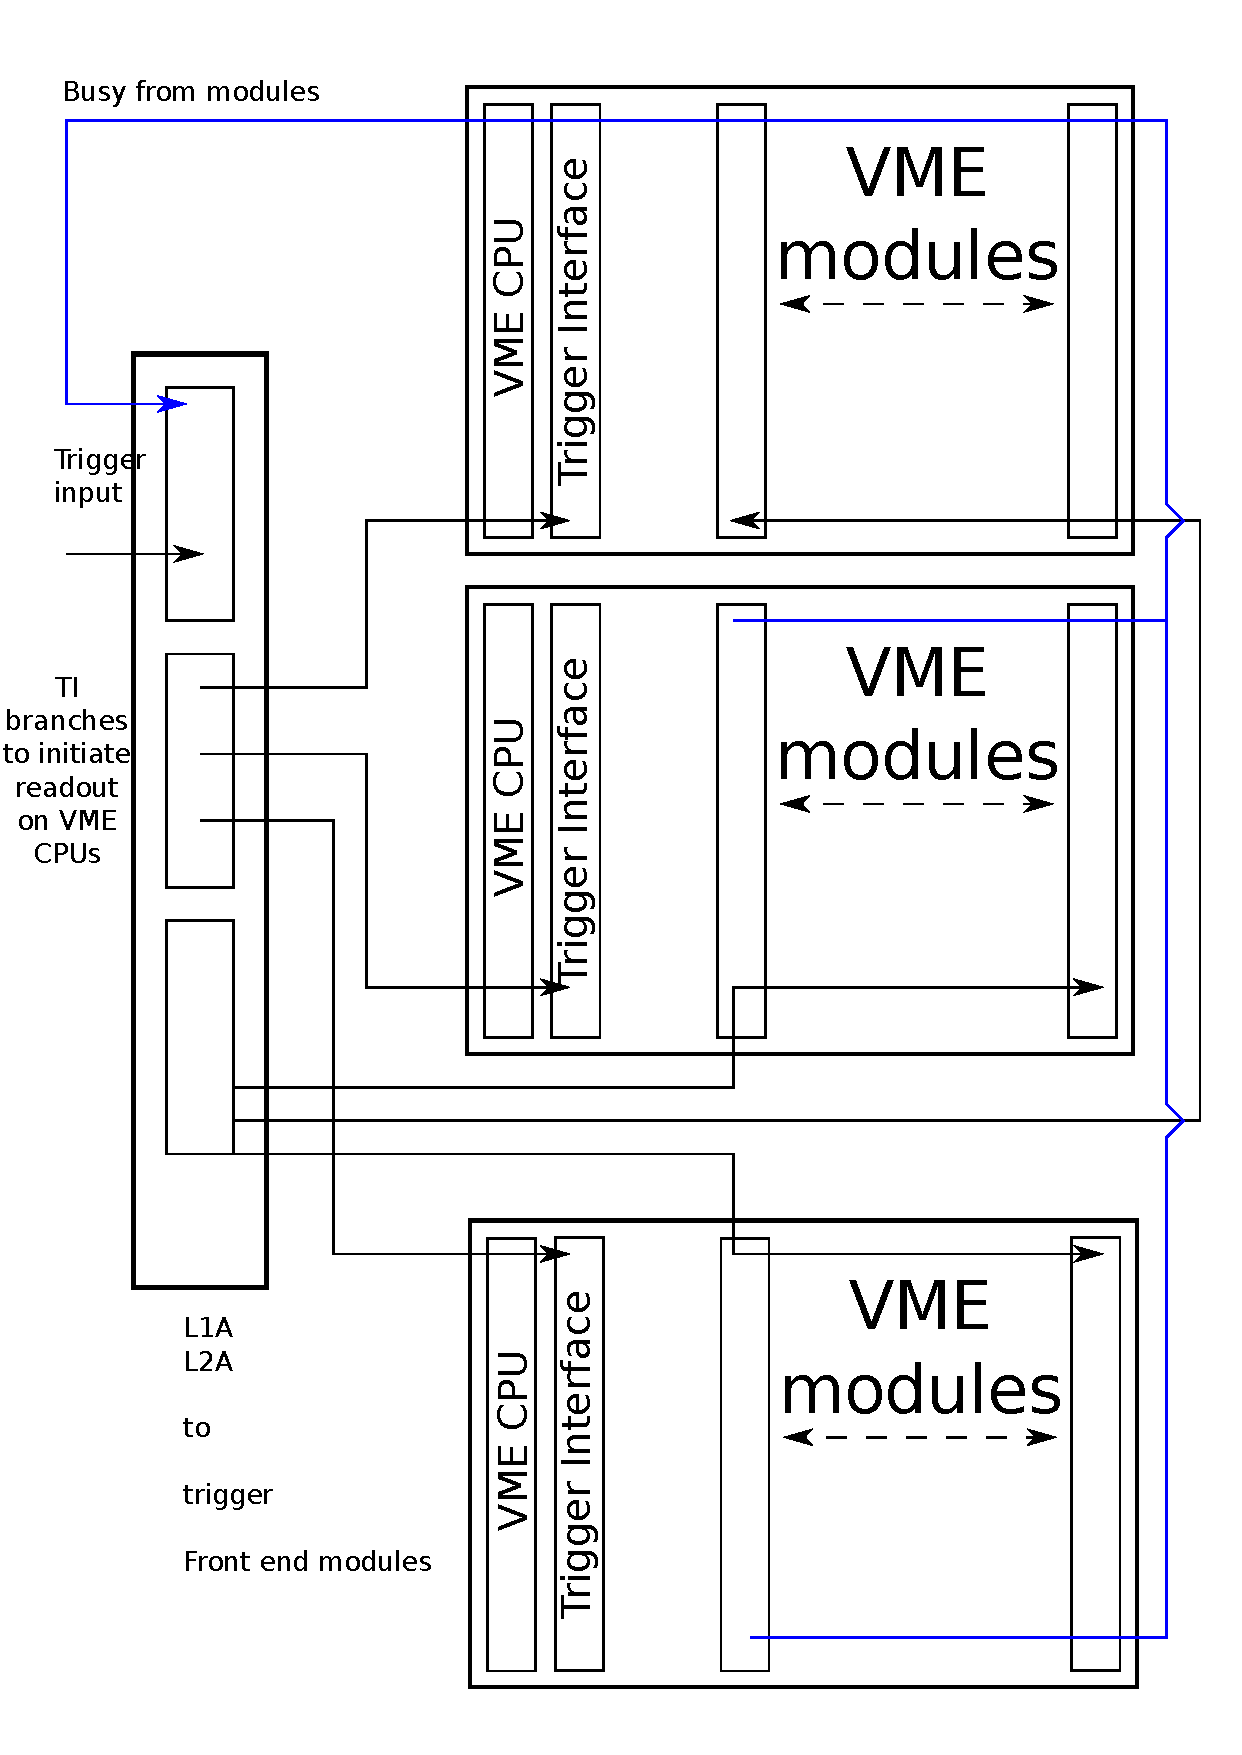
\includegraphics[scale=0.55]{figs/TS.pdf}\\
\caption{\label{fig:TS} Standard CODA configuration}
\end{figure}

\subsection{NINO amplifier discriminator boards }
The discriminator card (Fig. \ref{fig:nino-schematic}) is based on
the NINO chip \cite{NINO}, shown schematically in the blue-shaded
box of Fig\ref{fig:nino-schematic}. NINO was designed originally
for time of flight systems at the ALICE experiment. It is an 8-channel
CMOS ASIC which accepts differential input signals and provides LVDS
output signals for timing. The output width is dependent on the charge
of the input signal and may be stretched by an amount, dependent on
the voltage applied to pin 9. This is currently 1.25~V, which stretches
by 10~ns. The threshold is set by applying a differential DC voltage
to pins 47 and 49. Pin 47 is fixed at 1.25~V and 49 is varied between
1.25~V (zero threshold) and 1.90~V (maximum). Ref. \cite{NINO}
specifies that the threshold range is 10-100~fC and for the present
application this translates to a voltage levels in the few-mV range.
\begin{figure}[h]
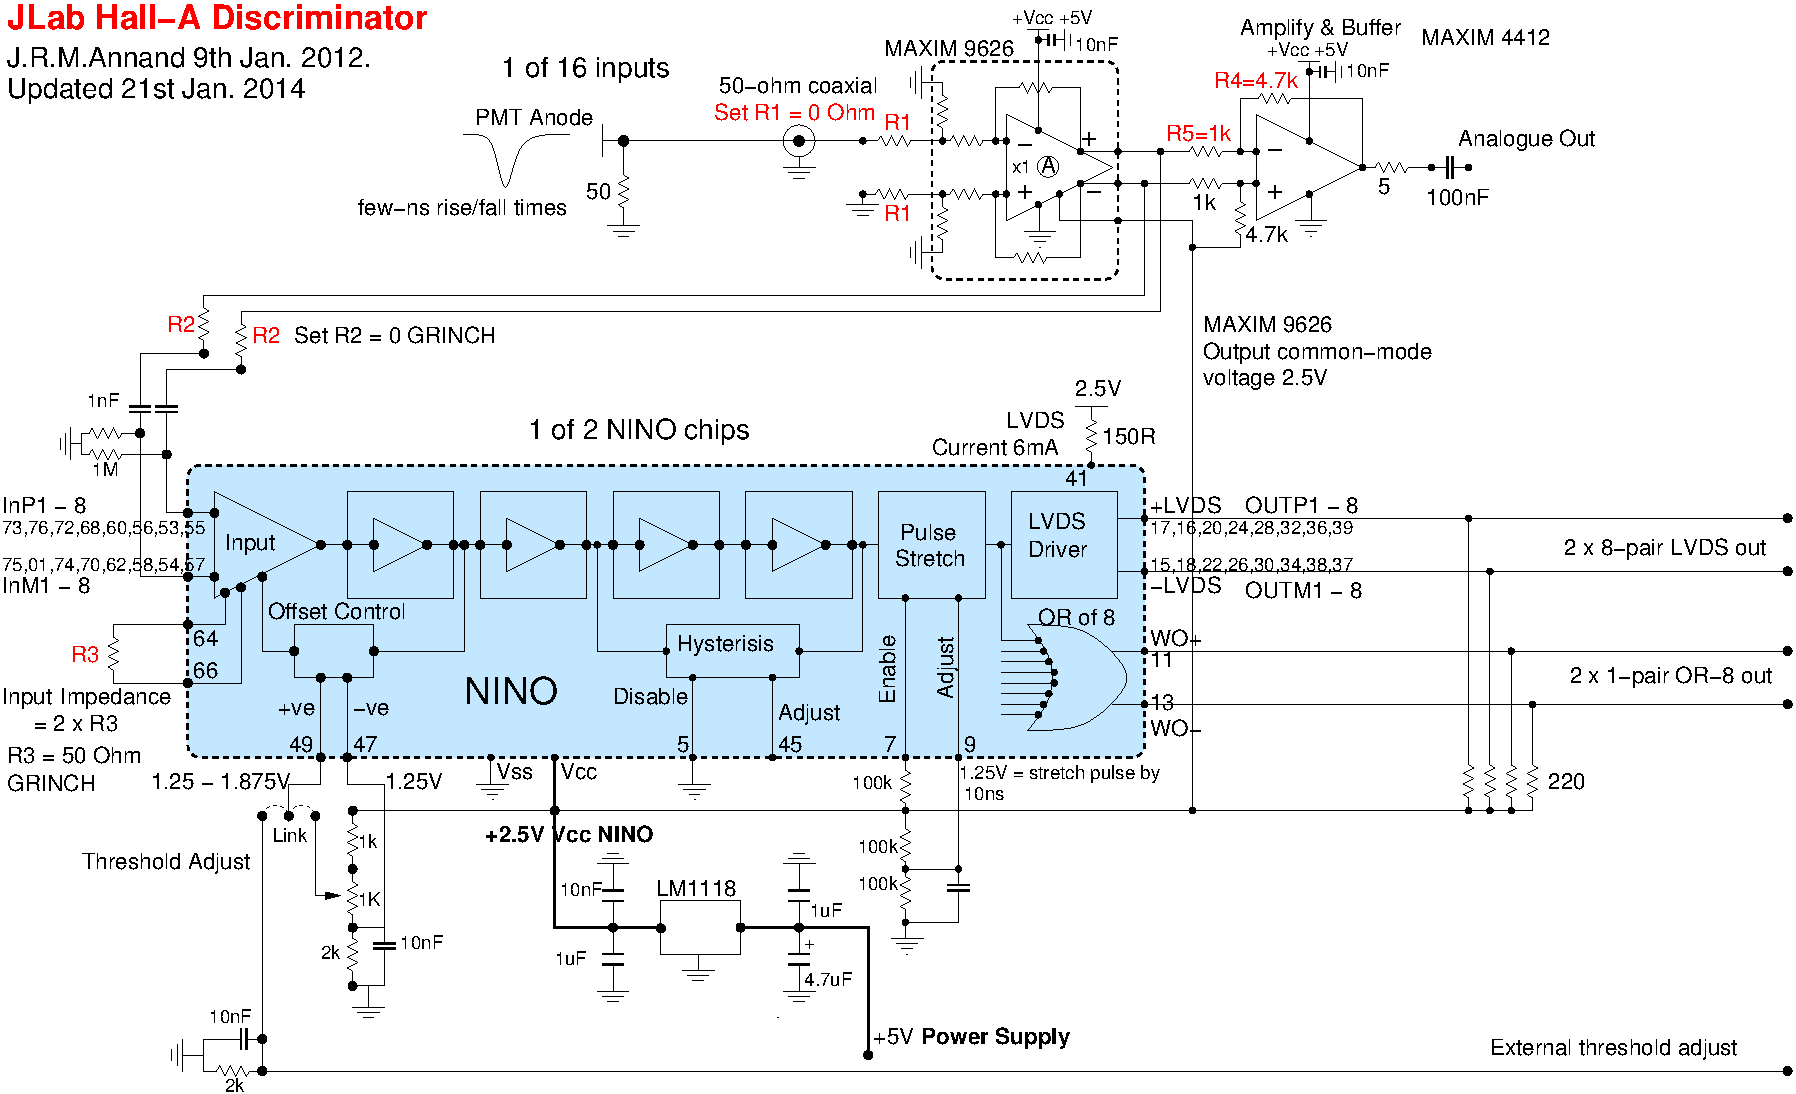
\includegraphics[width=1\columnwidth]{NINO/ReportJan14/CherenkovNINO-4}

\protect\caption{\label{fig:nino-schematic}Circuit diagram of the discriminator card.
A schematic diagram of the NINO chip is shown in the area shaded blue.}


\end{figure}
For Hall-A/SBS experiments, the discriminator card will be used with
PMT so that a front-end circuit is required to convert the input signal
from single ended to differential. This is implemented using the MAXIM
9626, which is a unity-gain, low-noise, low-distortion, fully-differential
amplifier, with a bandwidth of 1.35~GHz. Resistors R1 allow the input
impedance to be tuned to the input transmission line and for 50~$\Omega$
coaxial cable R1 = 0~$\Omega.$ The differential output from the
MAXIM 9626 feeds to the NINO input via capacitors which block the
common-mode voltage offset applied to the input circuit. Resistors
R2 can potentially be used to provide some attenuation of the pulse
(to vary the threshold range), but for GRINCH R2 = 0~$\Omega.$ Resistor
R3 sets the input impedance of NINO and the current value of 50~$\Omega$
sets the impedance to 100~$\Omega.$

The front end also provides a buffer amplifier, suitable to drive
charge digitizing hardware. This is required to calibrate the non-linear
relation between time-over-threshold and pulse amplitude. It is implemented
using the MAXIM 4412 operational amplifier, which is moderately fast
and relatively inexpensive. The gain is $(1+R4/R5)$, nominally a
factor 5.7.

Fig.\ref{fig:nino-photo} is a photograph of the Mk-IV prototype card.
Components are mounted on a 5-layer PCB, designed and manufactured
by ZOT Integrated Manufacturing based
in Musselburgh, Scotland. Components are surface mounted, but for
the NINO chips standard solder masking techniques did not give a reliable
connection to the PCB, due to the fine pitch of the pads. The ``balling''
technique, whereby precise quantities of solder are deposited on the
pads, solved this problem. The card is designed for stand-alone operation
(i.e. it does not reside in an electronics crate), so that it can
be mounted close to the detector using the four mounting points at
the corners of the card. The printed circuit board houses 2 Mk1 (8-channel)
NINO chips, associated front-end amplifier circuitry, connectors for
input signals and connectors for output analogue and LVDS logic signals.
Input cables can be connected, either by the $16\times2$-pin arrangement
shown in Fig.\ref{fig:nino-photo}, or alternatively hard soldered
to the card. Provision of a connector to allow cables to be routed
parallel to the plane of the card is to be implemented on future production
versions of the card. The output connectors are standard 17-pair,
0.1'' pitch IDC, commonly used with ECL logic.

\begin{figure}[h]
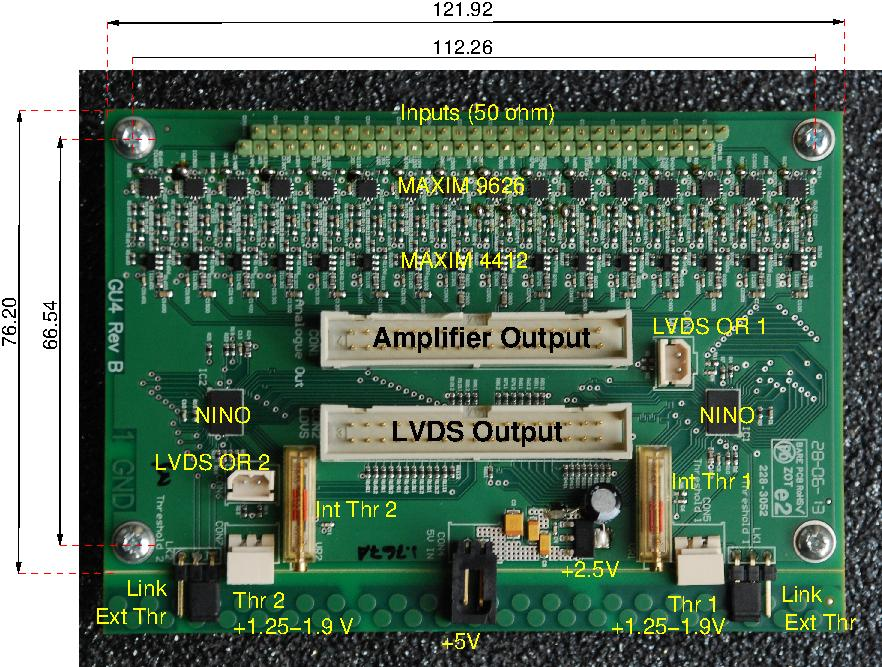
\includegraphics[width=1\columnwidth]{NINO/ReportJan14/NinoCardPhoto}

\protect\caption{\label{fig:nino-photo}The NINO-based amplifier-discriminator card.
Dimensions are in mm. Displayed is a prototype board. GRINCH and hodoscope
cards will have type-MCX coaxial connectors.}
\end{figure}


The card operates from a single +5V supply which powers the operational
amplifiers and a voltage regulator which supplies 2.5~V to the NINO
chips. The amount of current drawn on the 5~V line is 1.25~A. Discriminator
thresholds can be adjusted by on-board potentiometers, or alternatively
from an external voltage source. This is chosen by the position of
the jumpers on the ``Link Ext Thr'' pins attached at the bottom
left and right of the PCB. As shown, the PCB has been configured to
operate with external voltage thresholds, supplied via the ``Thr1''
and ``Thr2'' connectors at the bottom of the card. When mounted,
the card will be covered by a metal sheet to shield from electromagnetic
disturbance and will include attachments to clamp input and output
cables in place.

The NINO will be readout using Fastbus 1877S TDCs.

\subsection {GEM readout}
\subsubsection{APV25}
The GEM readout is carried out by the APV25 chip. It is a 128 channels ASICs with pipeline depth of 192 samples sampling at 40 MHz giving a pipeline depth of 4.8 $\mu s$ ( limited to 4 $\mu s$ for the hardware to perform correctly) . When a trigger is issued the corresponding cells are frozen until they are readout while the other cells are still being used reducing the dead time.
For each trigger all the data of 128 channels are transferred at 40 MHz rate in a multiplexed analog format. Adding some header and event information 141 words are transmitted for each trigger which gives a transfer time of $141x25 ns = 3.6 \mu s $. In case of high background several consecutive time samples can be sent in order to detect pile up, we plan to read 3 samples which gives a transfer time of 10.8 $\mu s$. This allows dead-timeless operation for rates up to 90 KHz.

\subsubsection {Multi Purpose Digitizer (MPD)}
 The readout planned to be used the the INFN Multi Purpose Digitizer (MPD). It is a VME board with a 200 MHz FADC and signals to control the APV setup and readout. It has 2 ports which can read up to 8 APVs each for a total of 16 APVs giving 2048 channels. 
For the GEp trackers 14 APVs will be read per MPDs, the APV data is 130 24 bit words so the event size to be transferred for 3 samples is then :

$130 ( words per APV ) * 3 (samples ) * 14 (APV ) * 3 (bytes ) = 16.38 KB $

Several readout schemes are possible with the MPD. The board complies with the VME64X standard and can transfer up to 200 MB/s in sustained rate using the VME320 protocol on the VME64X backplane \ref{OldMPD}. 

\begin{figure}
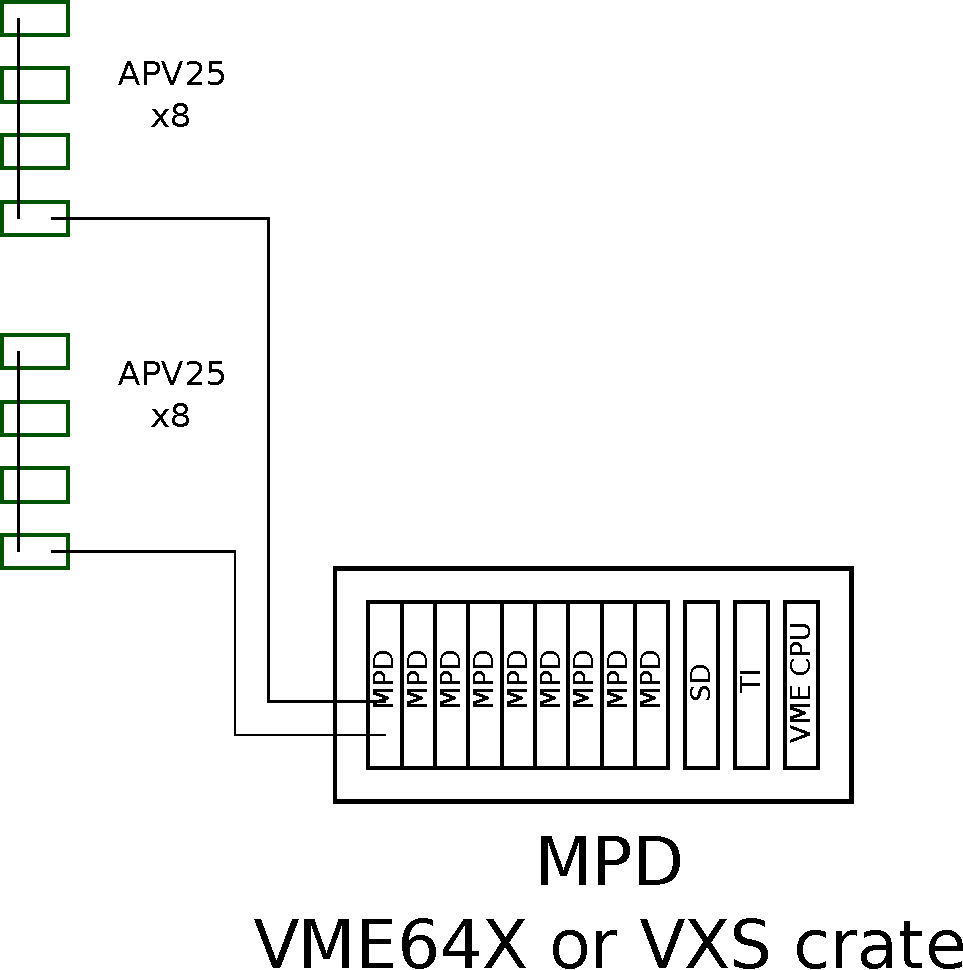
\includegraphics[scale=0.55]{figs/OldMPD.pdf}\\
\caption{MPD readout using VME64X backplane}
\label{OldMPD}
\end{figure}
When taking into account trigger processing and overhead of the DMA transaction, we reach an actual sustained sustained rate of about 100 MB/s.

At the assumed maximum rate of 5 KHz ( expected is 3 KHz ), that gives a raw data rate of 81.9 MB/s going into one single MPD from the APVs.
In the case of the GEp5, it was estimated that occupancy was around 60\% which would corresponds then to 49.2 MB/s per MPD after zero suppression which would give 2 MPDs per crates. 
To reduce the data the deconvolution algorithm will be implemented on the MPD to improve the timing resolution and reduce the occupancy by effectively shortening the pulse by applying a weighted sum similar to the on board deconvolution of the APV25 \cite{French:2001xb} to the multiple consecutive samples recorded, we expect a factor of at least 3 reduction of the accidental background. Doing the deconvolution on the MPDs allows to have more flexibility in processing the data and is expected to have better performance than the onboard one.

If the data reduction factor is not sufficient to transfer through the standard VME backplane, we can also transfer the data through VXS port or through the optical link of the MPD to allow parallel transfer of the data.
In order to further reduce the cost and amount of data recorded on tape a new readout scheme was proposed taking advantage of the JLAB electronics and optical link feature of the MPD. All the MPDs\ref{NewMPD} are sending data in parallel to the SSP and the SSP reduced the area of interest to be recorded using geometrical informations from othe HCAL and ECAL.
\begin{figure}
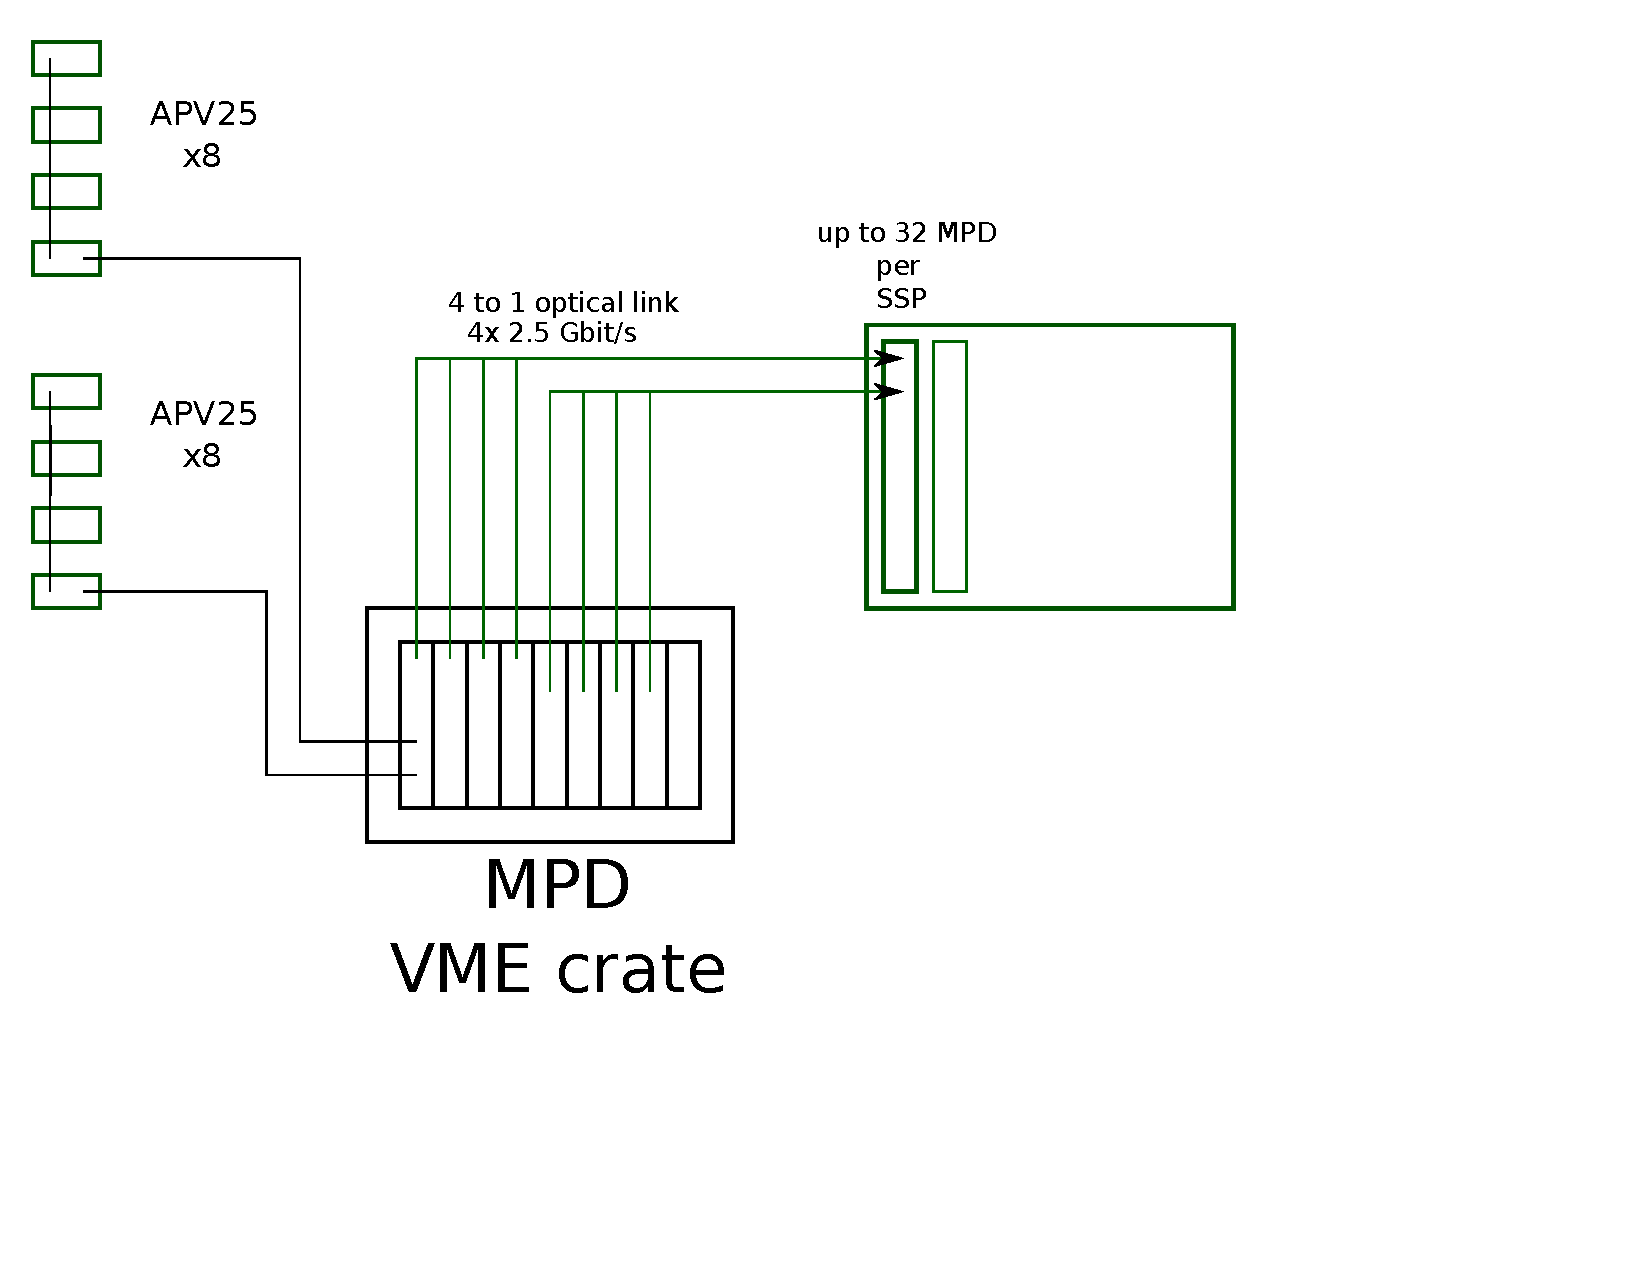
\includegraphics[scale=0.55]{figs/NewMPD.pdf}
\caption{MPD readout using optical link readout}
\label{NewMPD}
\end{figure} 

The MPD has 2 inputs to receive the trigger and an optional external clock. One output of the MPD will have the board busy signal to be used to inhibit the trigger in case the MPD buffers are filling up or if an APV raises an error condition.

\section{Pipelined electronics HCAL trigger}
\label{sec:hcal-vxs}
The hadron calorimeter will be read out by the JLAB pipelined electronics.
The central module for this system is the JLAB FADC250, a 16-channel 12-bit FADC sampling at 250~MHz. The input signals are continuously recorded into the memory with a memory depth up to 8 us. The system is thus dead timeless as long as the trigger is generated before the memory rolls over and the event of interest is overwritten.
The Flash ADC has two separated data path.
The first one uses the new high speed serialized VME standard called VME switched Serial (VXS).
It allows full duplex point to point connection at up to 2.5 Gbps per lane using the backplane central connector.
Currently the FADC is using two VXS lanes giving 5 Gbps of bandwidth.
This allows to transfer a 16 bit word from each FADC to a Crate Trigger Processor (CTP) board every 4~ns.
Each FADC being connected to The CTP via a 5 Gbps VXS link, the CTP uses up to 16 FADC words from each FADC to form a 32-bit word every 4~ns which can be a lower resolution sum of all the channels or a bit pattern of the channel hit for example.
The CTP board then sends the processed signals to a Sub-System Processor (SSP) board via a 10 Gbps optical link which puts together all the data from individual crates and computes the associated quantities which will be used in the trigger.
All the SSP boards send their processed information to a Global Trigger Processor (GTP) which will produce the calorimeter trigger.
Once a trigger is generated, the full resolution data which is still in the pipeline is readout out using the VME320 protocol at an average data rate of 200 MB/s.
The Flash ADC can run in different modes, it can either transfer all the samples of the waveform which can be useful to study pileup effect and background or process the data to give an integral over the length of the pulse. In both mode, a threshold can be put on each individual channel to reduce the data.

\begin{figure}
  \centering
  % Requires \usepackage{graphicx}
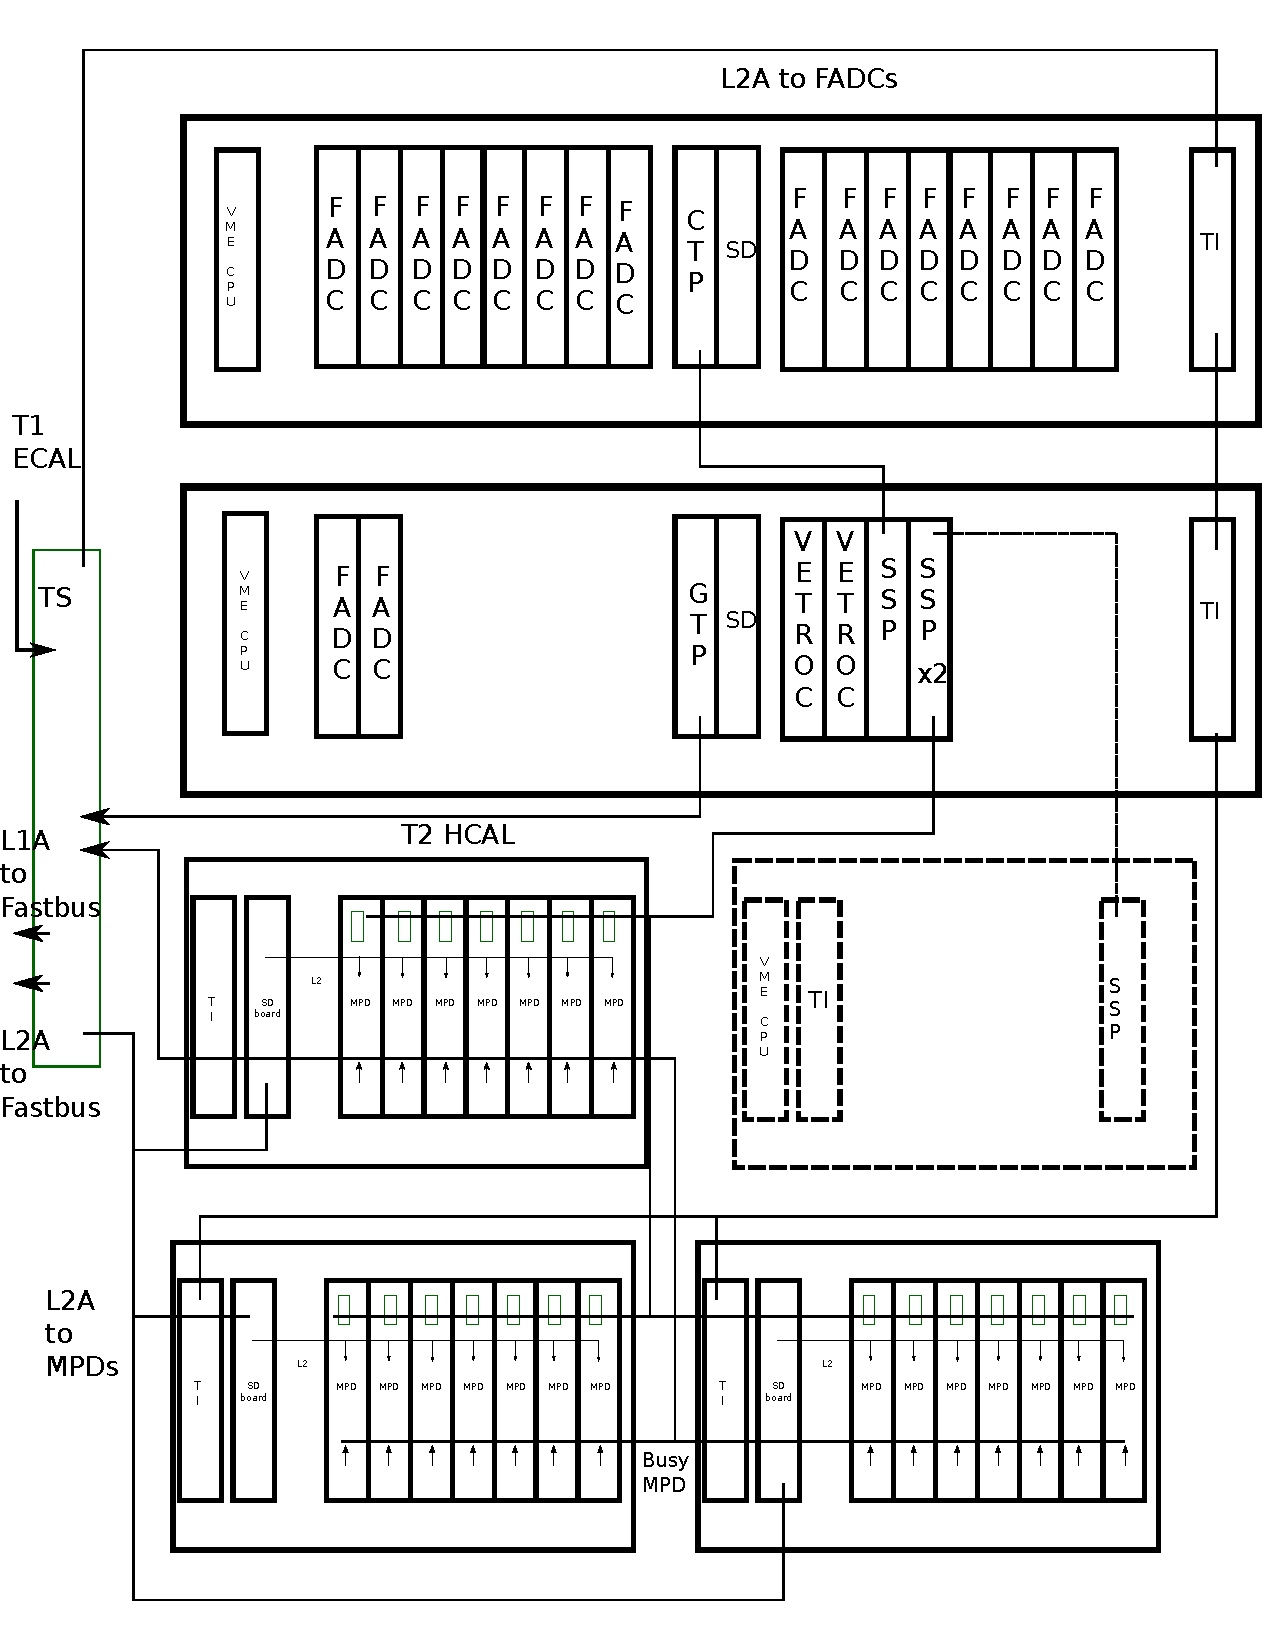
\includegraphics[width=\textwidth]{figs/NewMPDDetailed.pdf}\\
  \caption{Pipelined electronics configuration of HCAL with MPD readout through optical link}\label{fig:pipeline_daq}
\end{figure}

In order to be able to do the clustering, the scheme used for the Heavy Photon Search will be used.
Instead of sending a sum of all the channels every 4 ns, it uses frames of 32 ns. If a pulse is above threshold, the pulse is integrated over 32 ns for each FADC channel and the integral on 13 bit and a 3 bit time are packed into a word and sent to the CTP at 8 Gbps. At the end of the 32 ns frame, the CTP will have all the amplitudes of each FADC channels and will send them to the GTP using the optical link. 
The GTP having all the amplitude of all the calorimeter, it can compute all the sums of adjacent blocks.
A sum of 3$\times$3 blocks was implemented for the heavy photon search experiment (HPS) in Fig.\ref{fig:ClustHPS}.
In order to reduce the number of triggers coming from the background this summing approach is chosen to improve the online pion rejection.
A sum over 4x4 adjacent blocks can be implemented in the same way as the HPS scheme \ref{fig:HCALSum}. 

\begin{figure}
  \centering
  % Requires \usepackage{graphicx}
 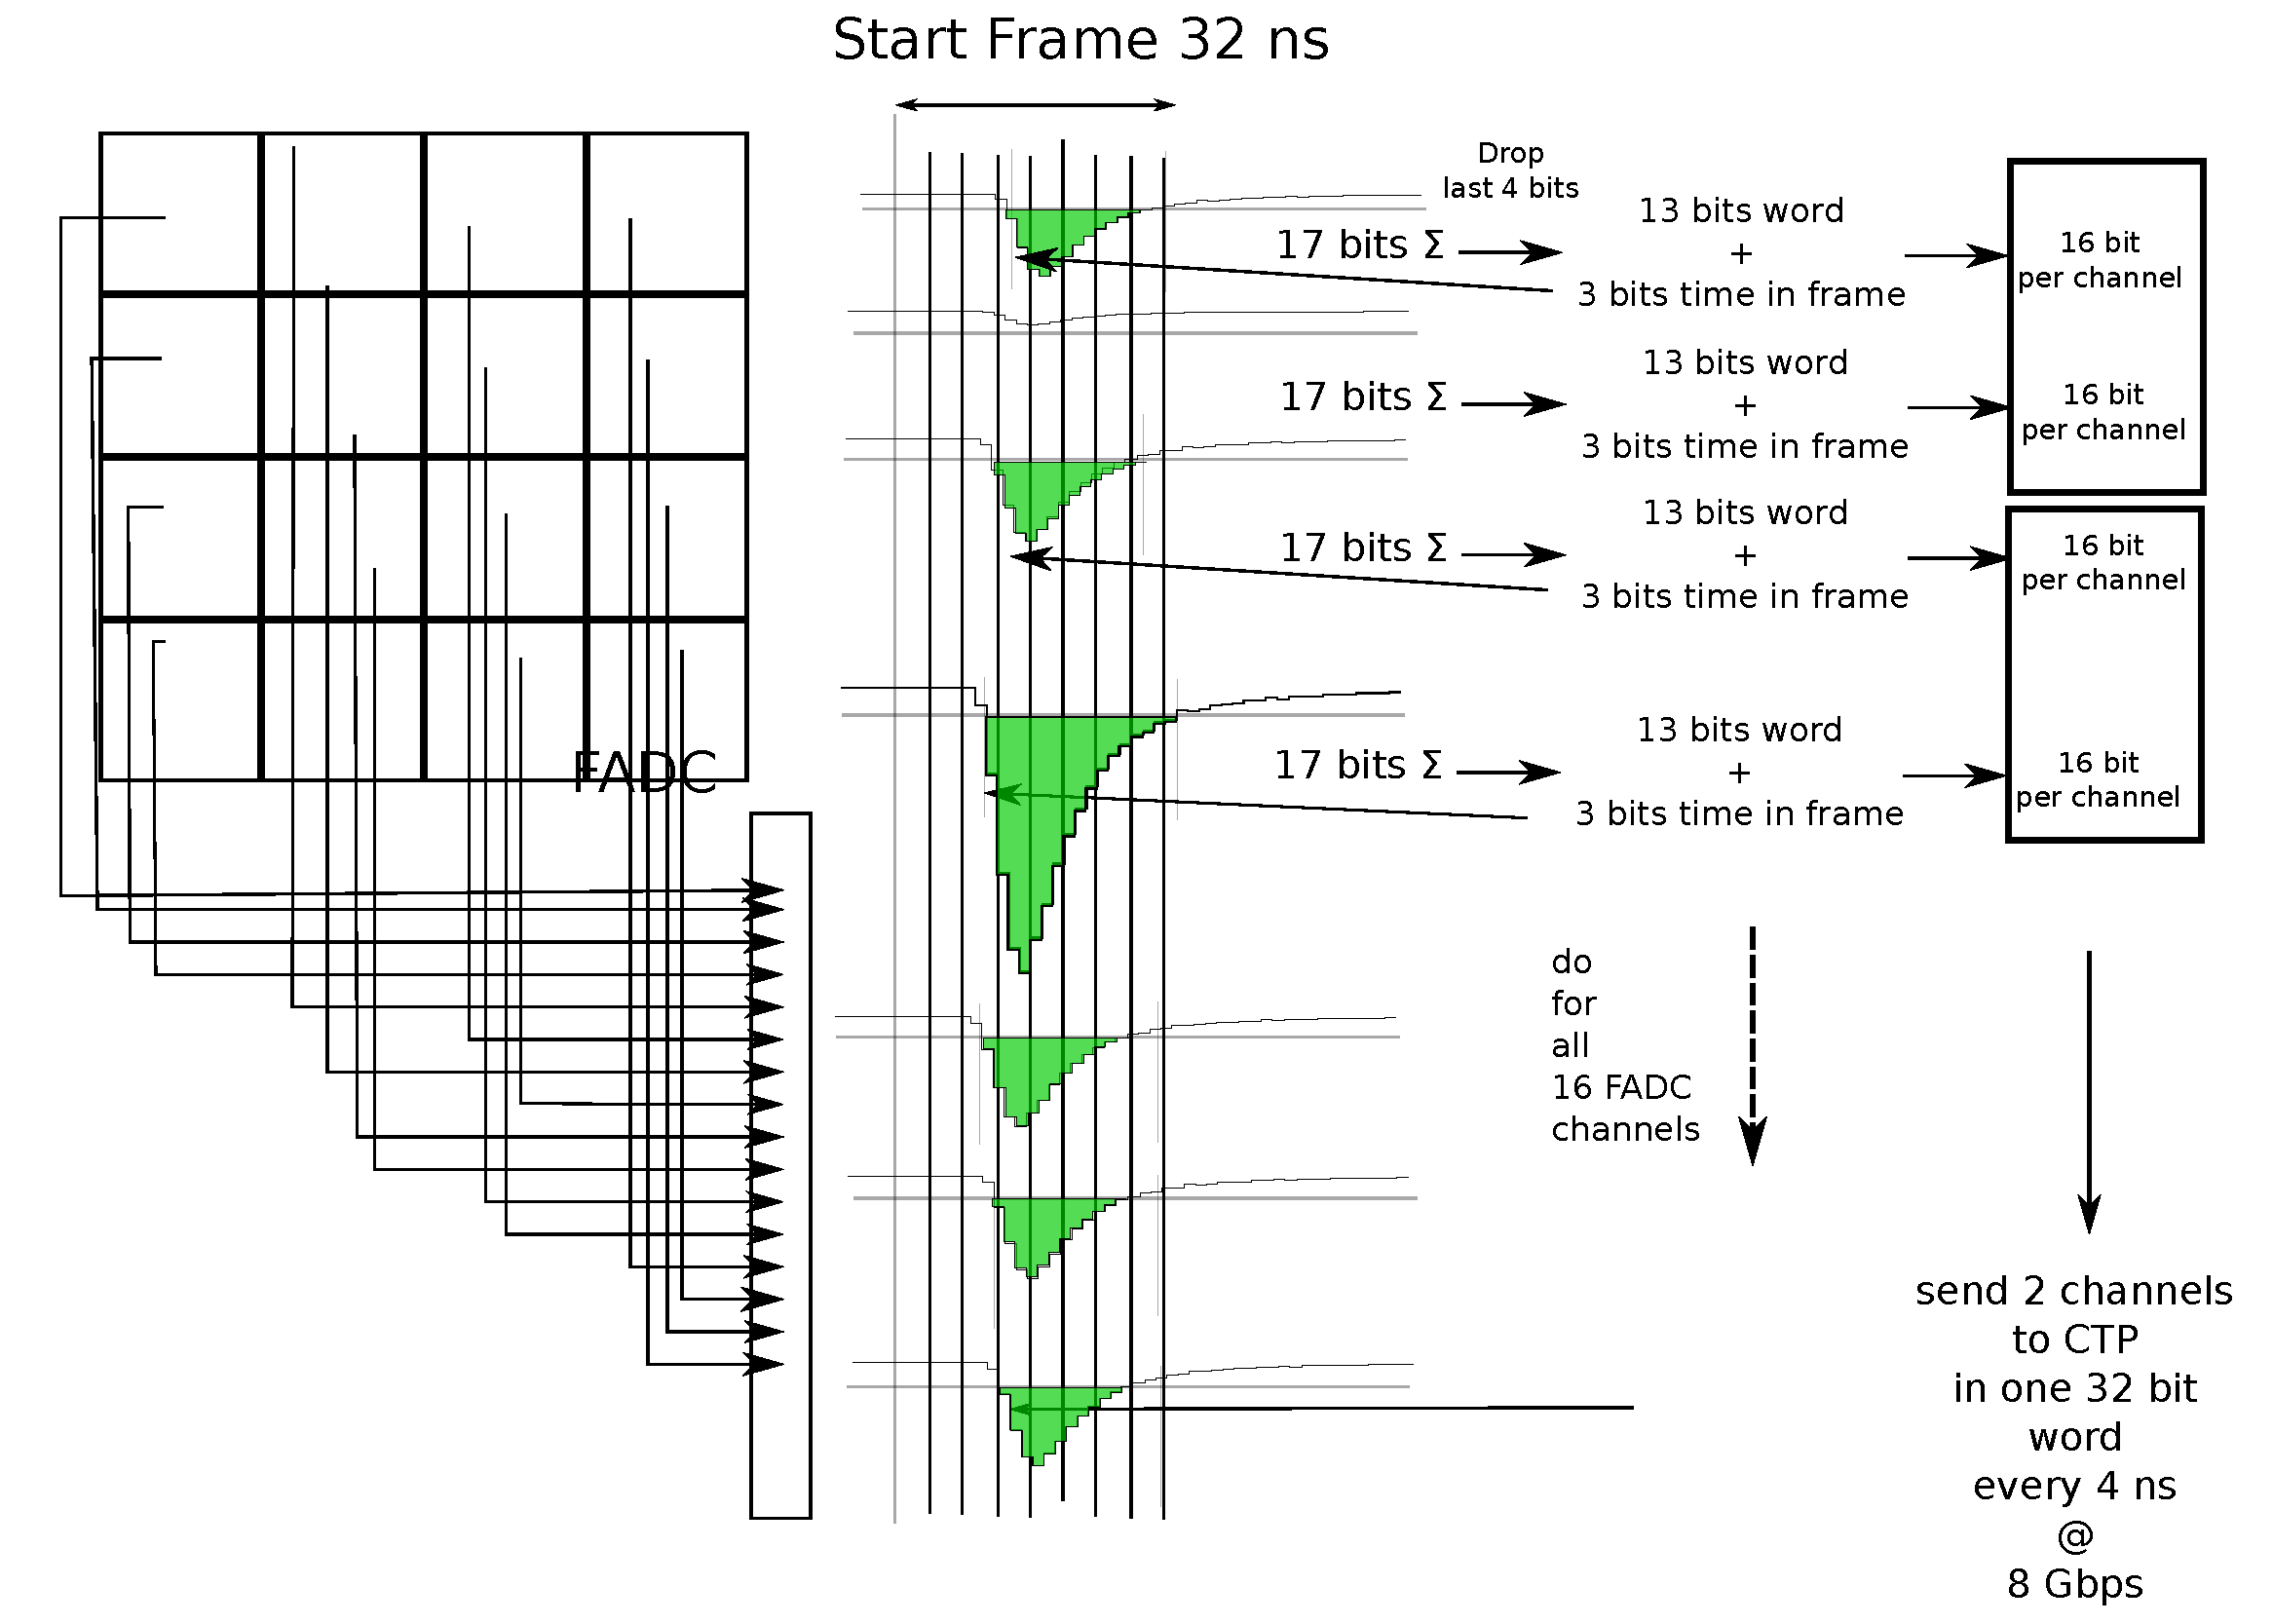
\includegraphics[width=\textwidth]{figs/CaloTrigger.pdf}
  \caption{Calorimeter clustering scheme using the HPS algorithm. All calorimeter signals are sent to the FADC. All 16 FADC channels integrals are sent to the CTP in 32 ns}\label{fig:ClustHPS}
\end{figure}


\begin{figure}
  \centering
  % Requires \usepackage{graphicx}
  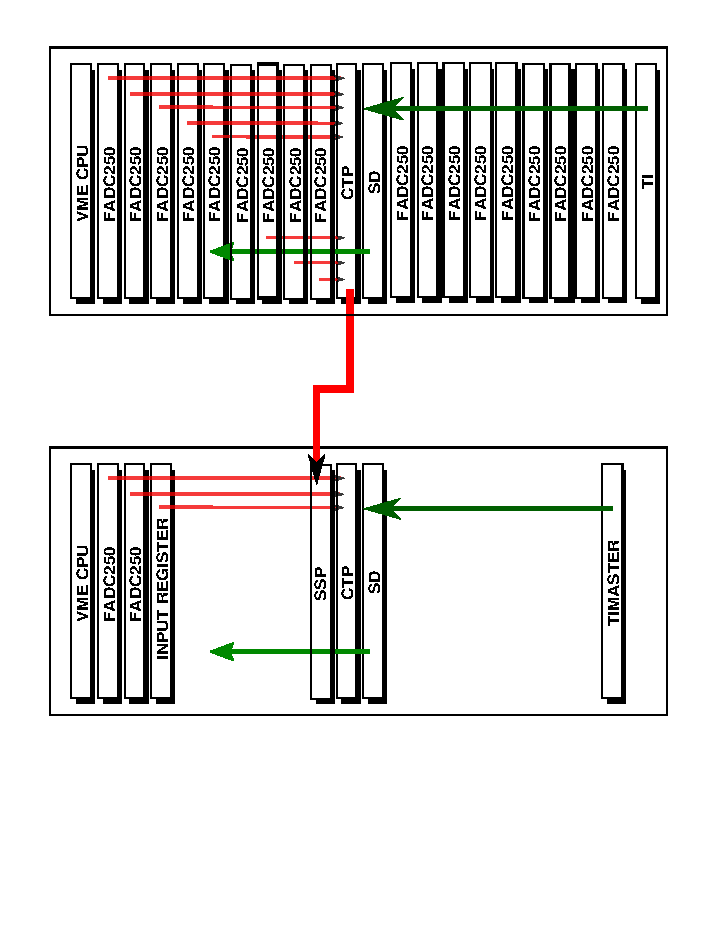
\includegraphics[width=\textwidth]{figs/VXSHCalFADC.pdf}\\
  \caption{HCAL crate layout }\label{fig:HCALFADC}
\end{figure}

\begin{figure}
  \centering
  % Requires \usepackage{graphicx}
 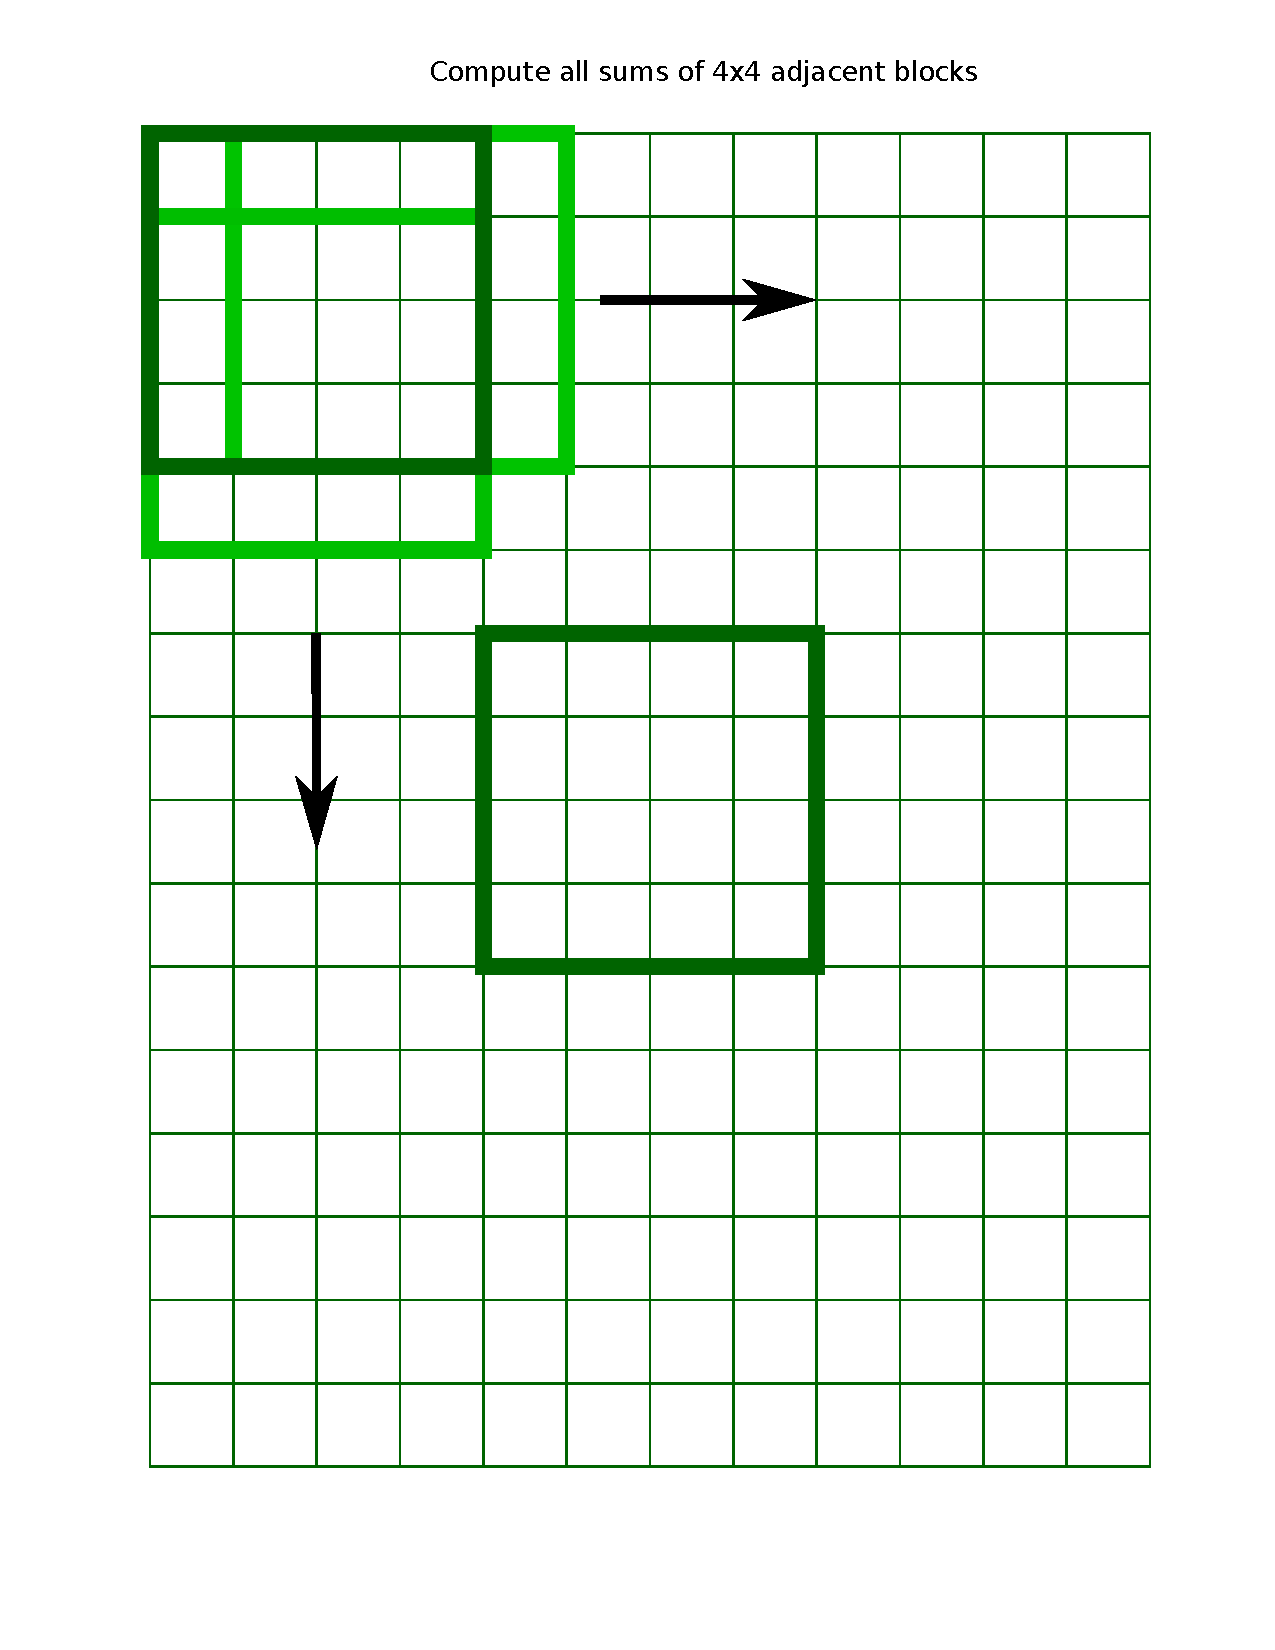
\includegraphics[width=\textwidth]{figs/HCALSum.pdf}
  \caption{All sum of 4x4 are computed, if one is above threshold L2 is generated }
\label{fig:HCALSum}
\end{figure}

Since we have 288 channels for the HCAL, 18 FADCs will be used using two VXS crates Fig.\ref{fig:HCALFADC}. The crate with all 16 FADCs will send its data ti the other CTP through the SSP using the 10 Gb/s optical link. The second crate will hold the two additional FADCs and a pipelined input register called VETROC which can have up to 208 logic inputs which a 1 ns timing resolution, to send the sums firing in the ECAL to the GTP to generate the L2 using the geometrical matching of the HCAL with the ECAL. The total process will not take more than 1 $\mu s$ which is sufficiently fast for the APVs which have a look back of 4 $\mu s$. The GEM readout \ref{fig:pipeline_daq} will also be done using the SSP in the second VXS crate, if the amount of data is larger than 100 MB/s to transfer and additonnal crate will be added to readout the SSP.



\subsection{Fastbus}
Fastbus is an electronics standard developed in the 1980's. It can transfer up to 10 Megawords per second with a 32 bit width which gives a maximum theoretical throughput of 40 MB/s which translates in usual sustained rate of 15 MB/s. If the amount of data is greater than 15 MB/s, the modules will be split between several crates allowing readout in parallel.
Since we have a lot of Fastbus equipment on hand. It will be used in order to reduce the costs for the large number of detectors channels. The main readout is the Lecroy ADC 1881M a 13 bit ADC, with a 9 $\mu$s encoding time in 12 bit resolution and 12  $\mu$s in 13 bit resolution. The 1881M features a fast clear and is ready to take another event after 1 $\mu$s. For signal requiring time measurement 1877S TDC will be used, they have 96 channels per module. It is multihit up to 16 hits with an event buffer of 8 events. It has an encoding time  1.7 $\mu$s plus 50 ns per hit per channel giving a maximum encoding time of 78 $\mu$. Both modules supports sparsification to reduce the non useful data before transfer.
For each Fastbus crate a Struck Fastbus Interface (SFI) is a Fastbus Master is controlled by a standard VME controller which allows to control the Fastbus modules through any VME CPU. It is needed in each Fastbus bin to control the Fastbus modules.

The L2 trigger will take 1 $\mu s$ to be generated and with the fast clear time we expect a L1 front end deadtime to be 2 $\mu s$.

In the case of the experiments using the BigBite spectrometer, ECAL will be simply replaced by the BigBite shower.
Each SFI can hold 2 VME boards, one slot is used for the VME CPU and the VME TI will be placed in the second slot.

\section{Fastbus implementation}

In order to improve the data transfer rate a large number of Fastbus crate is going to be used.
Right now we are planning to use 12 crates for the ECal \ref{fig:FastbusEcal} and 9 crates for the Coordinate Detector.
One main challenge for the standard Fastbus electronics is the GEp5 experiment where the L1A rate is going to be of the order of 200 KHz. The calorimeter trigger is expected to be generated in less than 1 $\mu$s and the ADCs requires 1 $\mu$s giving a front end deadtime of about 40 \% at 200 KHz which is not acceptable. In order to reduce the front end dead time, the signal will be passively split between 2 or 3 Fastbus modules, so that when a module is busy encoding the next one is triggered eliminating the front end busy from the Fastbus.
In order to do that a slightly modified scheme is used.
The main trigger coming from the ECAL, is sent to the main TS at around 200 KHz rate, the TS produce a prompt level 1 accept trigger which will be used to trigger the non pipelined electronics. The L1A is processed by a V1495 FPGA \ref{fig:FPGAFlip} board programmed as a prescaler, which take one signal input and split the signal between 2 or more output ( number programmable up to 8 and in our case 2 or 3 ).
\begin{figure}
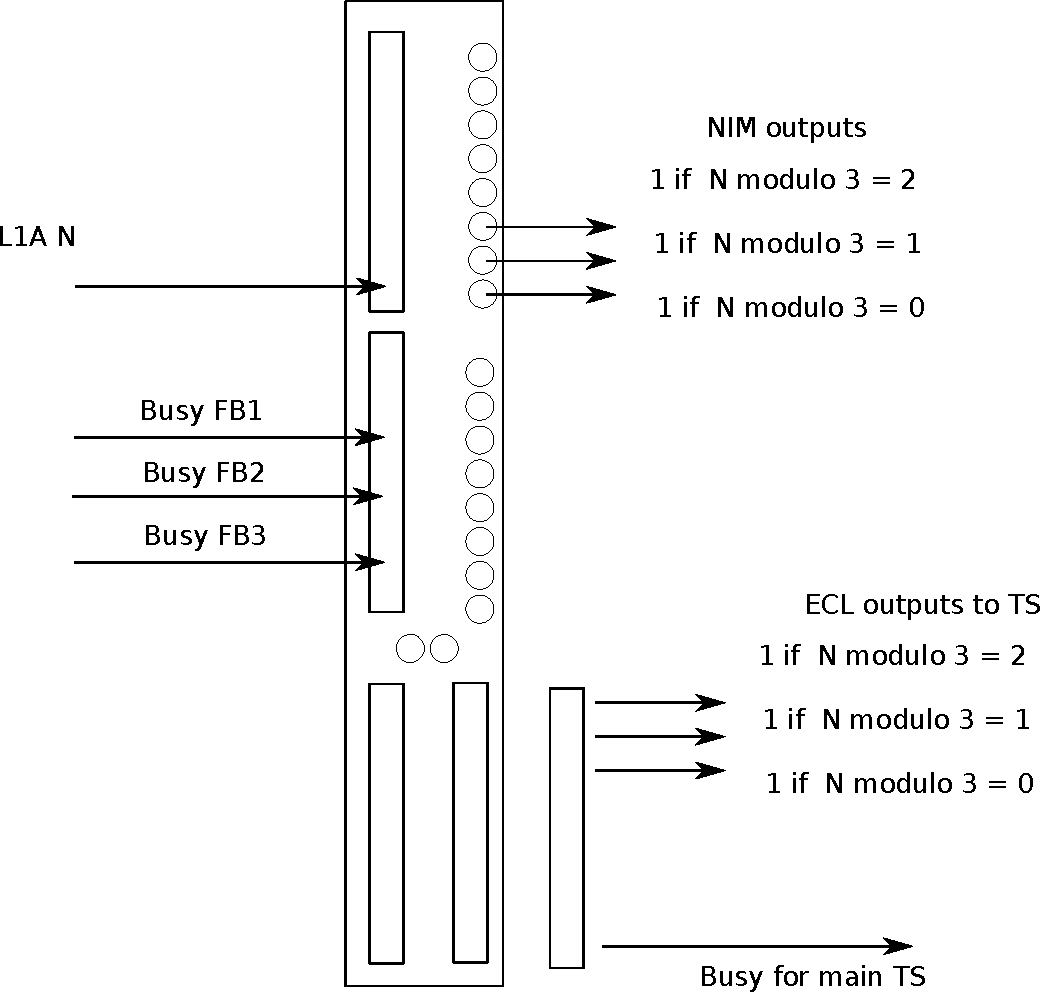
\includegraphics[scale=0.55]{figs/FPGAFlip.pdf}\\
  \caption{V1495 logic module programmed to distribute the L1A ( 200 KHz ) to the 3 different Fastbus DAQ}\label{fig:FPGAFlip}
\end{figure}
The board is programmed to cycle through its output. 
Three independent Fastbus setup will be in place with their own TS board \ref{fig:TSs} to keep each crates synchronized.
The busy signal of each setup will be sent to the V1495 which will generate a general busy signal sent to the main TS
to inhibit the trigger if the receiving Fastbus is not ready to receive a trigger. 
A common 250MHz clock will be sent from the pipelined electronics to scalers in each of the TS crate.
This will provide a timestamp to be used as an absolute reference for the time of an event.
A copy of the L1A of each system will be fed in each scalers giving a redundant check of the synchronization.

\begin{figure}
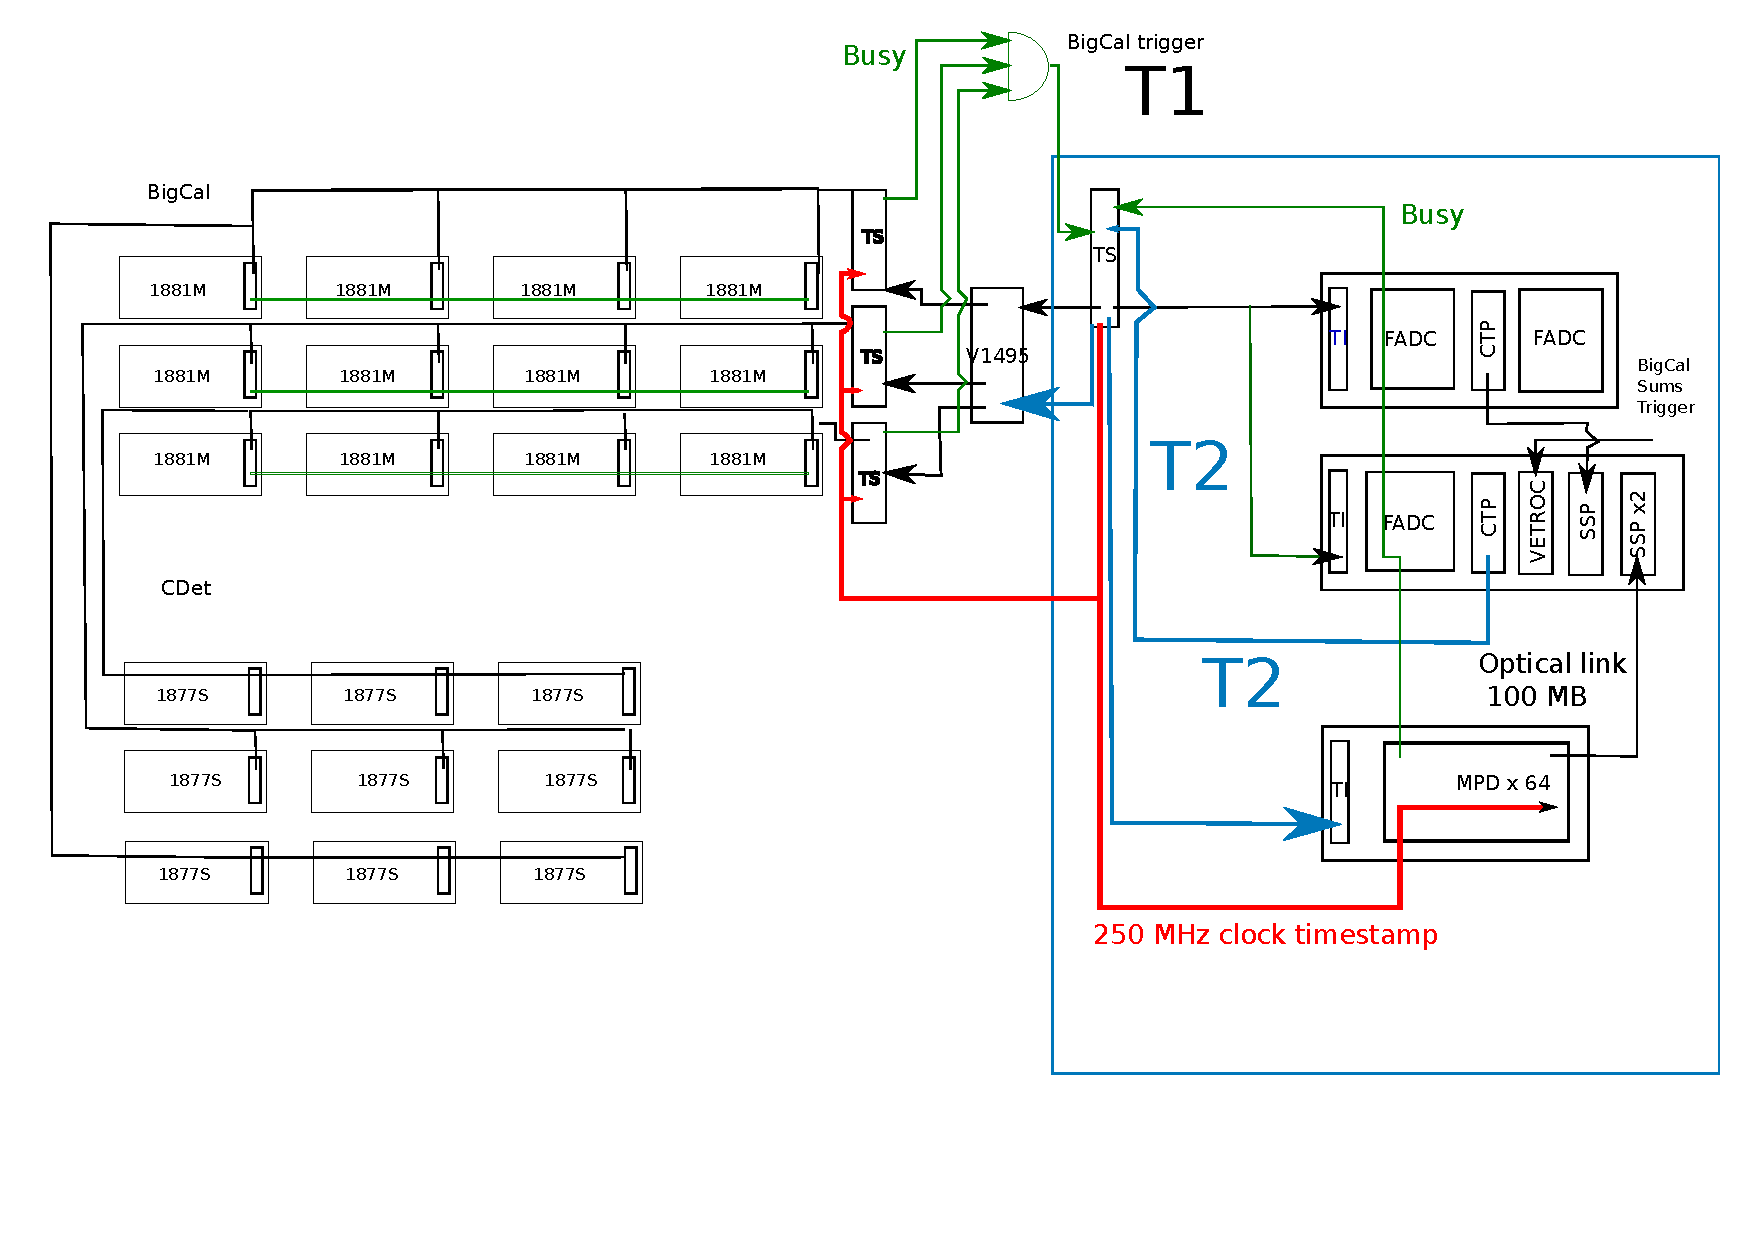
\includegraphics[scale=0.55]{figs/SBSlayoutOld.pdf}\\
  \caption{Full layout of the DAQ system}\label{fig:DAQLayout}

\end{figure}

\begin{figure}
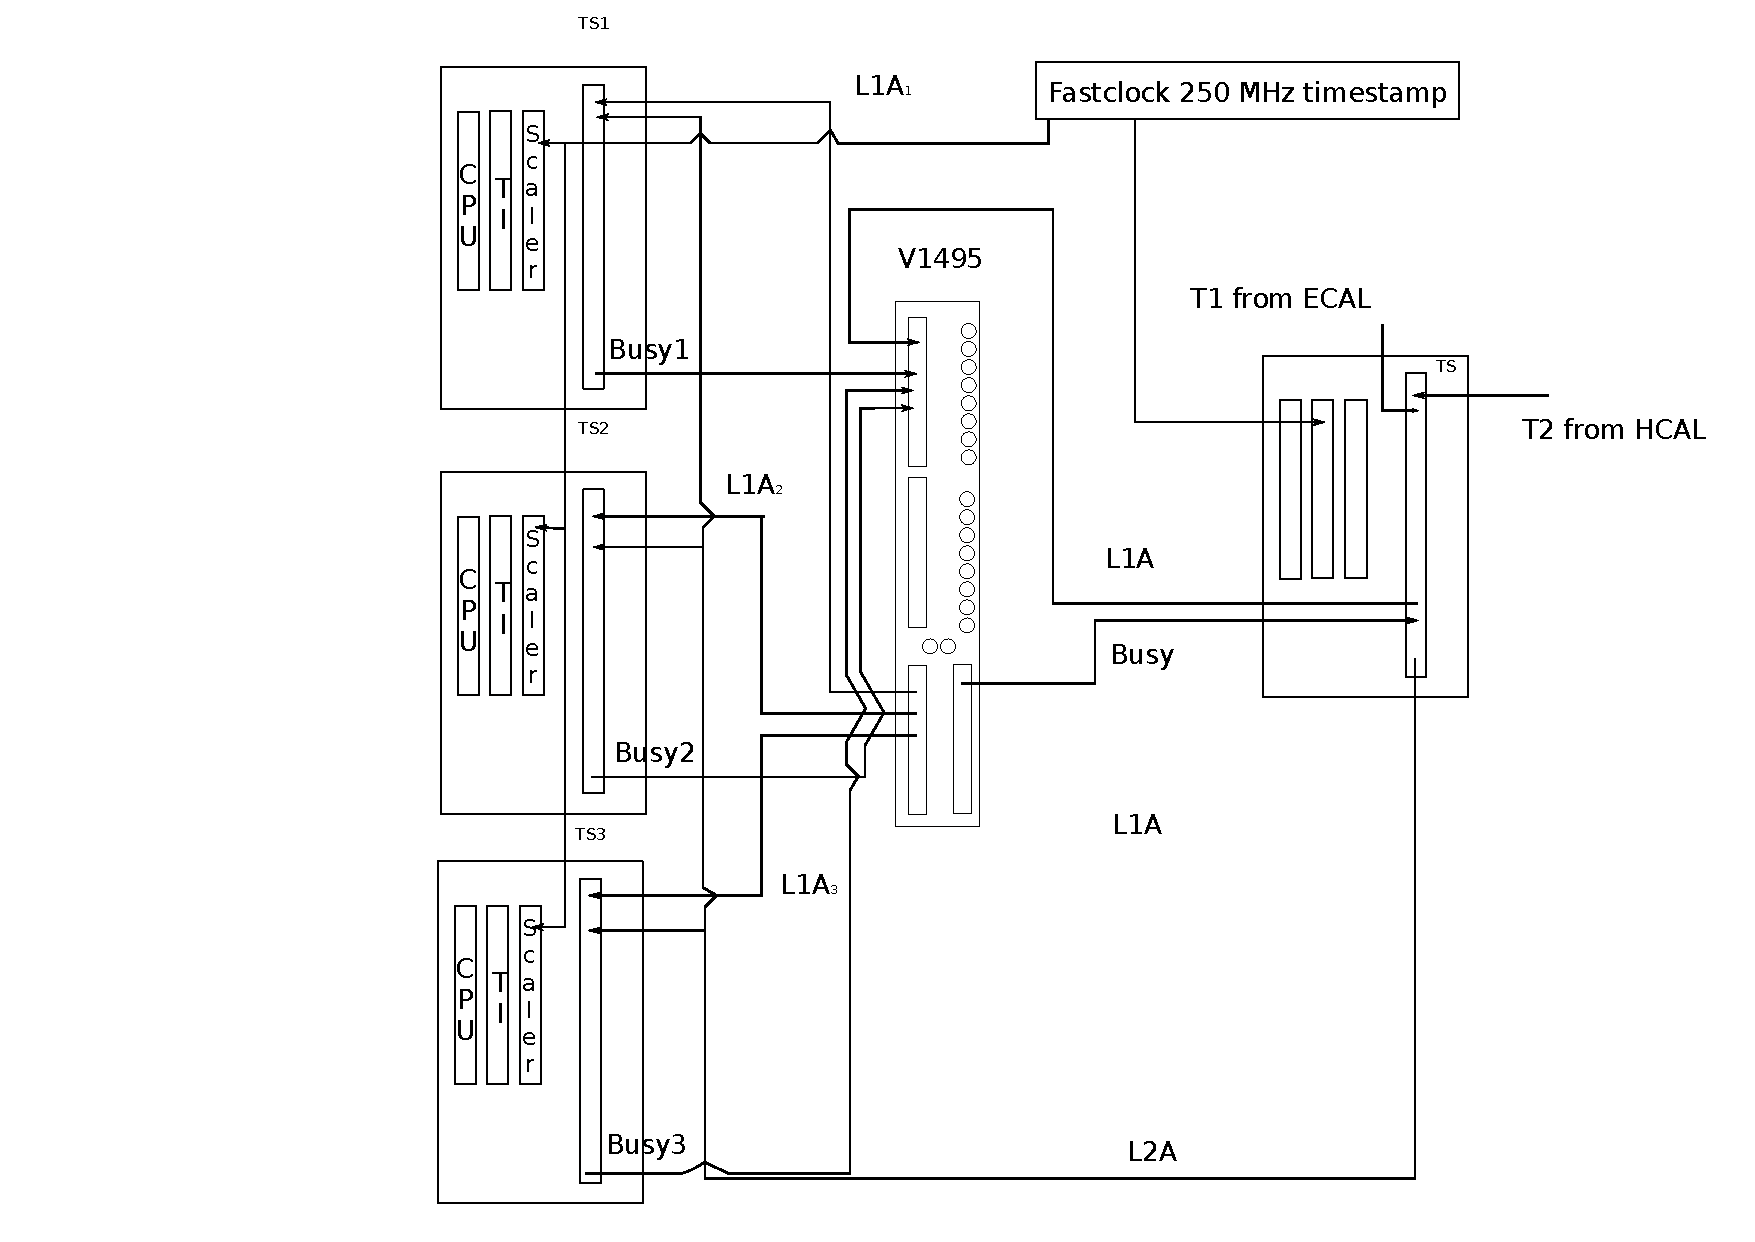
\includegraphics[scale=0.55]{figs/TSs.pdf}\\
  \caption{Zoom on the TS for each Fastbus subsystem}\label{fig:TSs}

\end{figure}

\begin{figure}
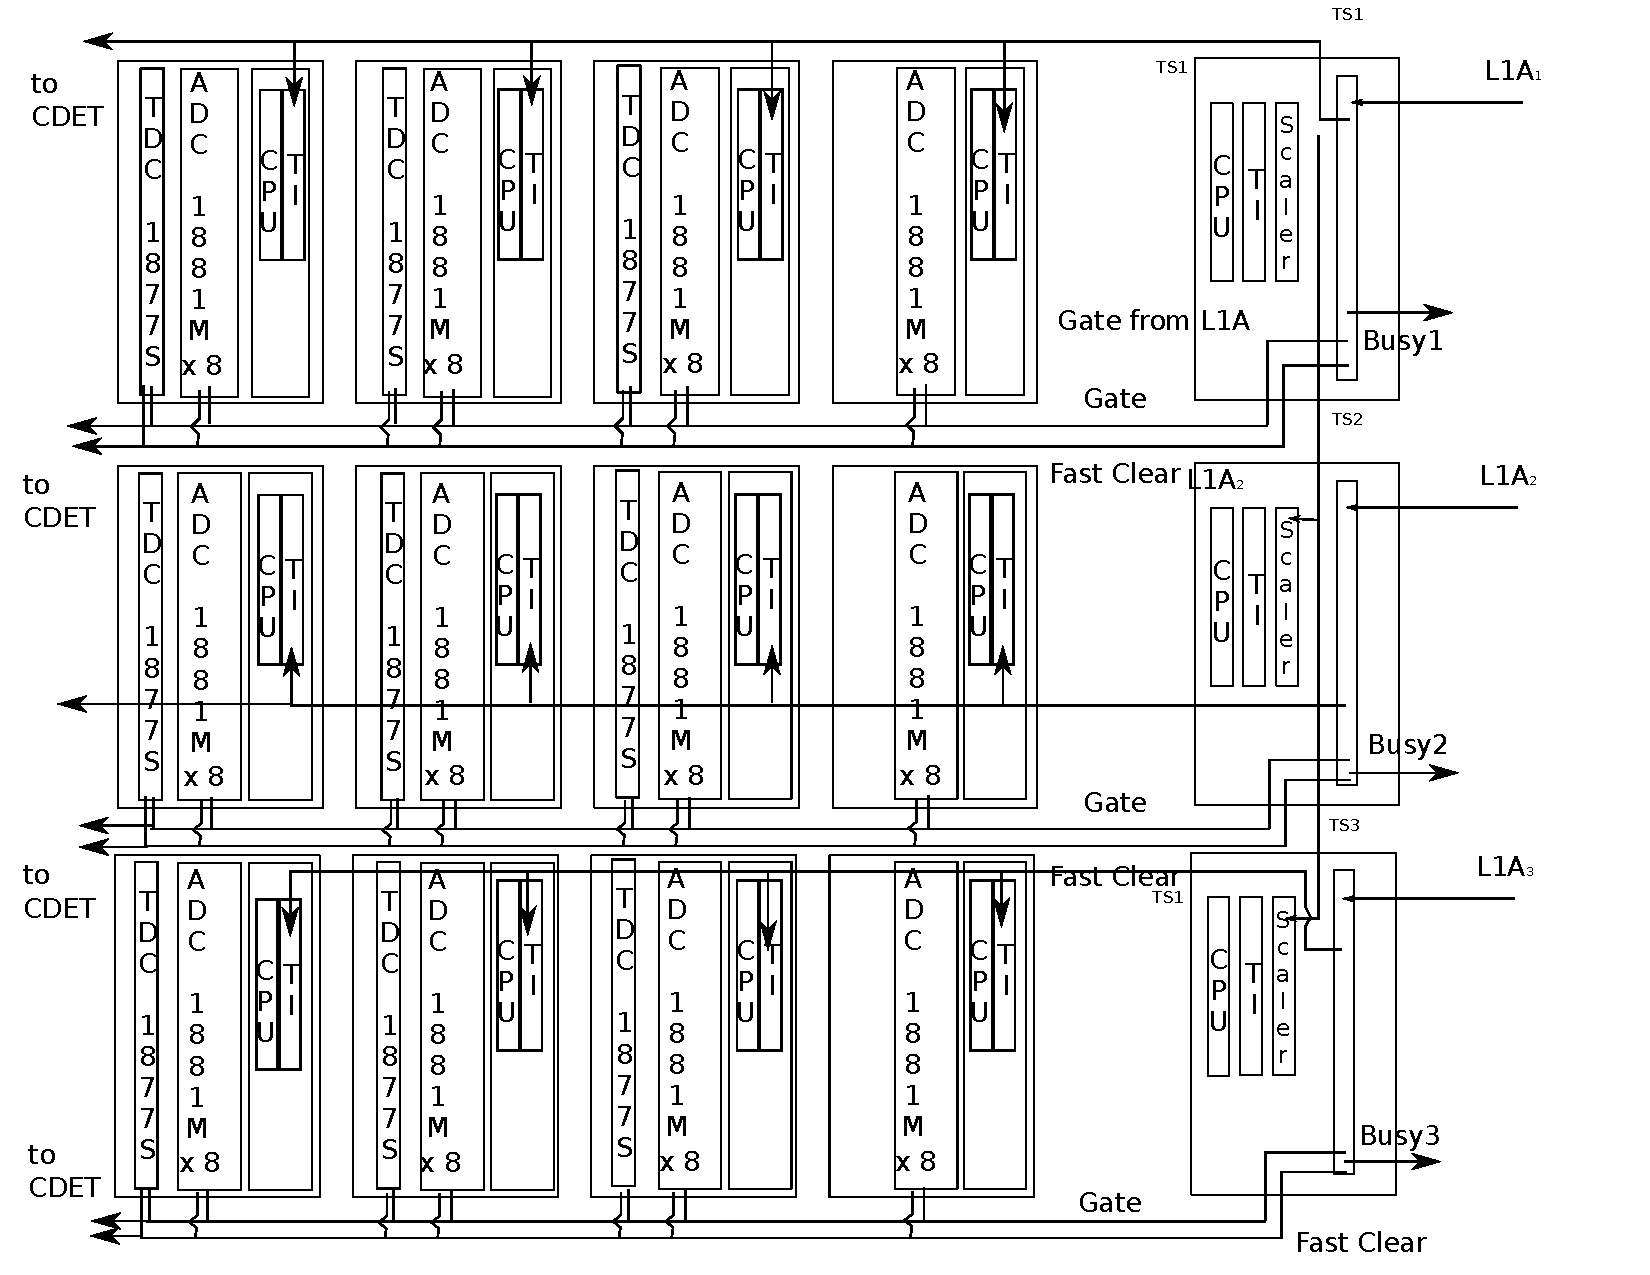
\includegraphics[scale=0.55]{figs/FastbusEcalDetailed.pdf}\\
  \caption{Fastbus ADC setup for ECAL }\label{fig:FastbusEcal}

\end{figure}
\begin{figure}
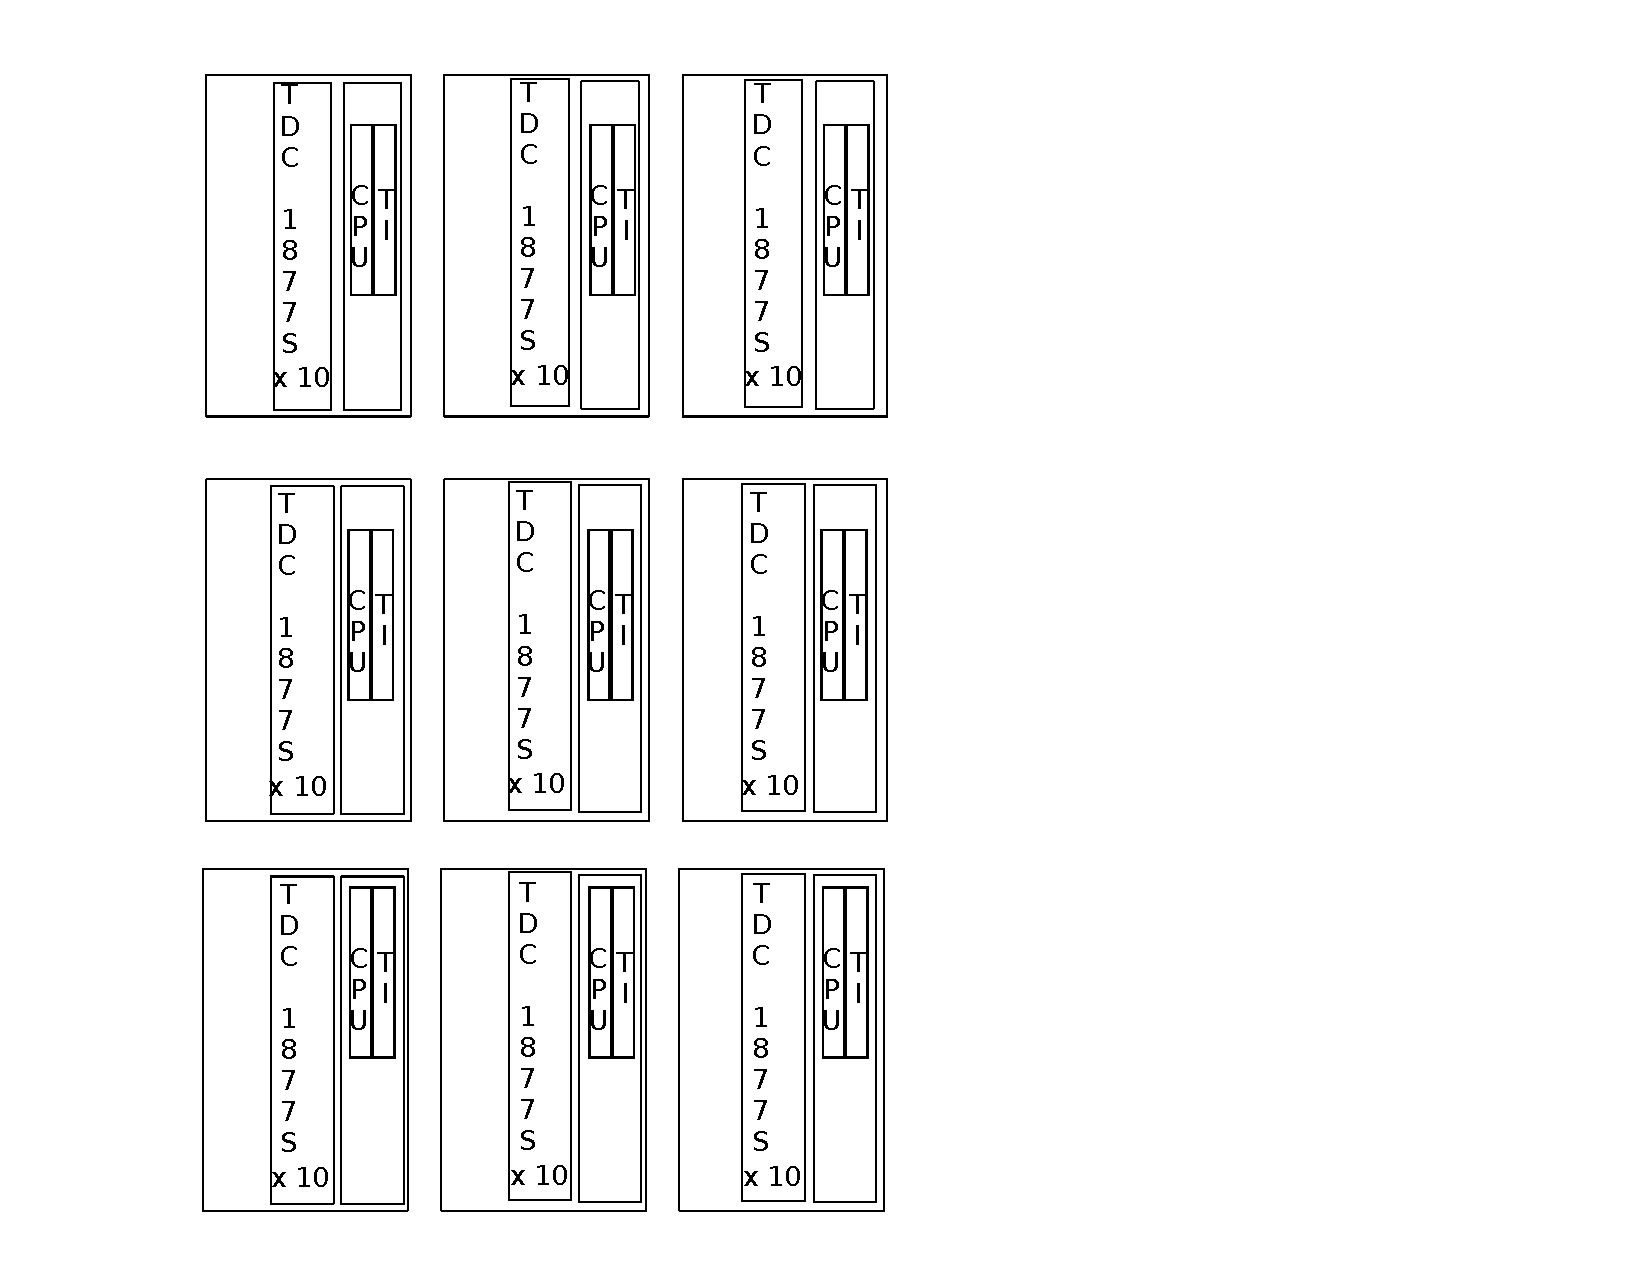
\includegraphics[scale=0.55]{figs/FastbusCDetDetailed.pdf}\\
  \caption{Fastbus TDC setup for CDet}\label{fig:FastbusCdet}

\end{figure}

The signals from the calorimeter are split to generate the trigger and a copy is sent through a 500 ns cable going into the Fastbus ADCs.
The ECAL trigger takes about 200 ns to be generated and is sent to TS with a high speed cable of about 10 meters long for an additional. Each TS stage takes 50 ns. Which leaves 150 ns to generate the gate for the Fastbus electronics.

Then the HCAL trigger is sent to the main TS after about 1 $\mu$s of processing to act as the L2 trigger \ref{fig:DAQLayout}. If the L2 occurs withing   1 $\mu$s the readout of the modules and the pipeline DAQ will start otherwise a fast clear is issue to the Fastbus and another trigger can be take 1 $\mu$s later reducing the front end dead time from the high L1 trigger rate.

Using this scheme the front end busy from the Fastbus will be reduced to 13 \% since the input rate for the Fastbus is reduced by a factor of 3.

The data streams from the Fastbus DAQs and the pipelined DAQ will be merged offline looking at the scalers and timestamp.

This setup will be used to readout ECAL or BigBite for the Neutron Form Factor experiments.
\section{GEp5 overview}
\subsection {ECAL calorimeter trigger}
\label{sec:ecal-trig}
 In the right   figure, the groups of 32 blocks are indicated connecting
group of 8 blocks by different colored squares. The group of 32 blocks overlap
by two groups of 8 in both horizontal and vertical directions. So most of the
groups of 8 have to go to 4 groups of 32. At the edges the groups of 8 feed into
two groups of 32. There are 204  groups of 32 are sums of 4 groups of 8 using
a 4 input channel linear FI/FO. The 228 groups of 32 would have to
go into discriminators.


\begin{figure}
  \centering
  % Requires \usepackage{graphicx}
  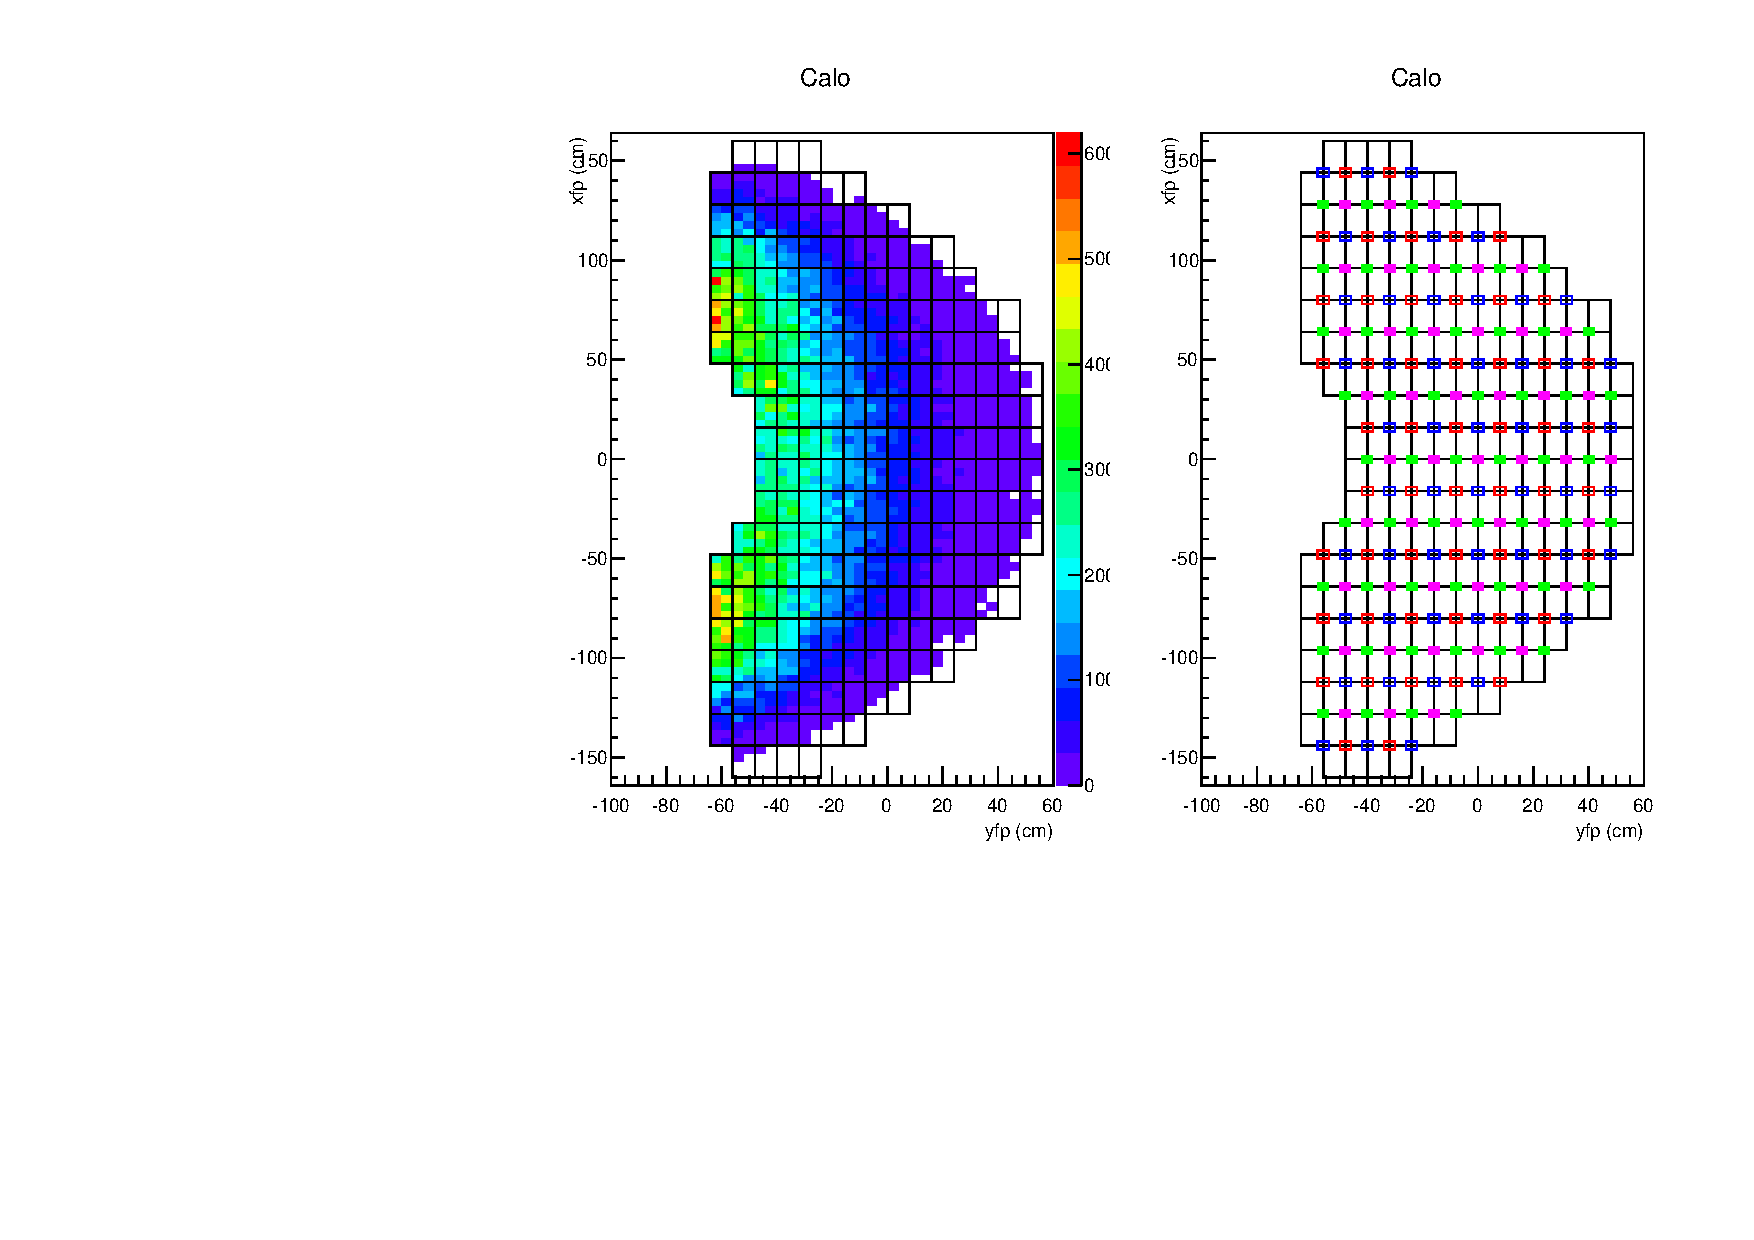
\includegraphics[width=\textwidth]{figs/cfpa.pdf}\\
  \caption{The left plot is the distribution of elastic electrons in ECAL with the black rectangles representing
groups of 2x4 lead glass blocks. The right plot demonstrates
the scheme for make overlapping groups of 32 lead glass blocks to be used in the ECAL trigger with
details explained in text.  }\label{fig:ECALTrig}
\end{figure}

The calorimeter trigger will be the fast L1 trigger for the Fastbus, it is generated in 200 ns. At the threshold of 80\% of the maximum energy, we foresee a maximum rate of 200 KHz.
The trigger will use the HCAL as L2 trigger, the singles rates in HCAL was estimated to be 2 MHz. The L2 trigger will be a cluster of 4x4 blocks over threshold and the L2 will also take as input the sums from the L1 to make a geometrical matching of ECAL and HCAL possible thanks to the overconstrained elastic kinematic. We expect to have a 3 KHz L2 coincidence trigger rate which will be used to trigger the FADC and GEM readout. 

\subsection {Overall setup}
An schematics giving an overview of the setup can be found in Fig.\ref{Gep5layout} and more details can be found in the experiment proposal E12-07-109: GEP/GMP \cite{GEpProp}
\begin{figure}
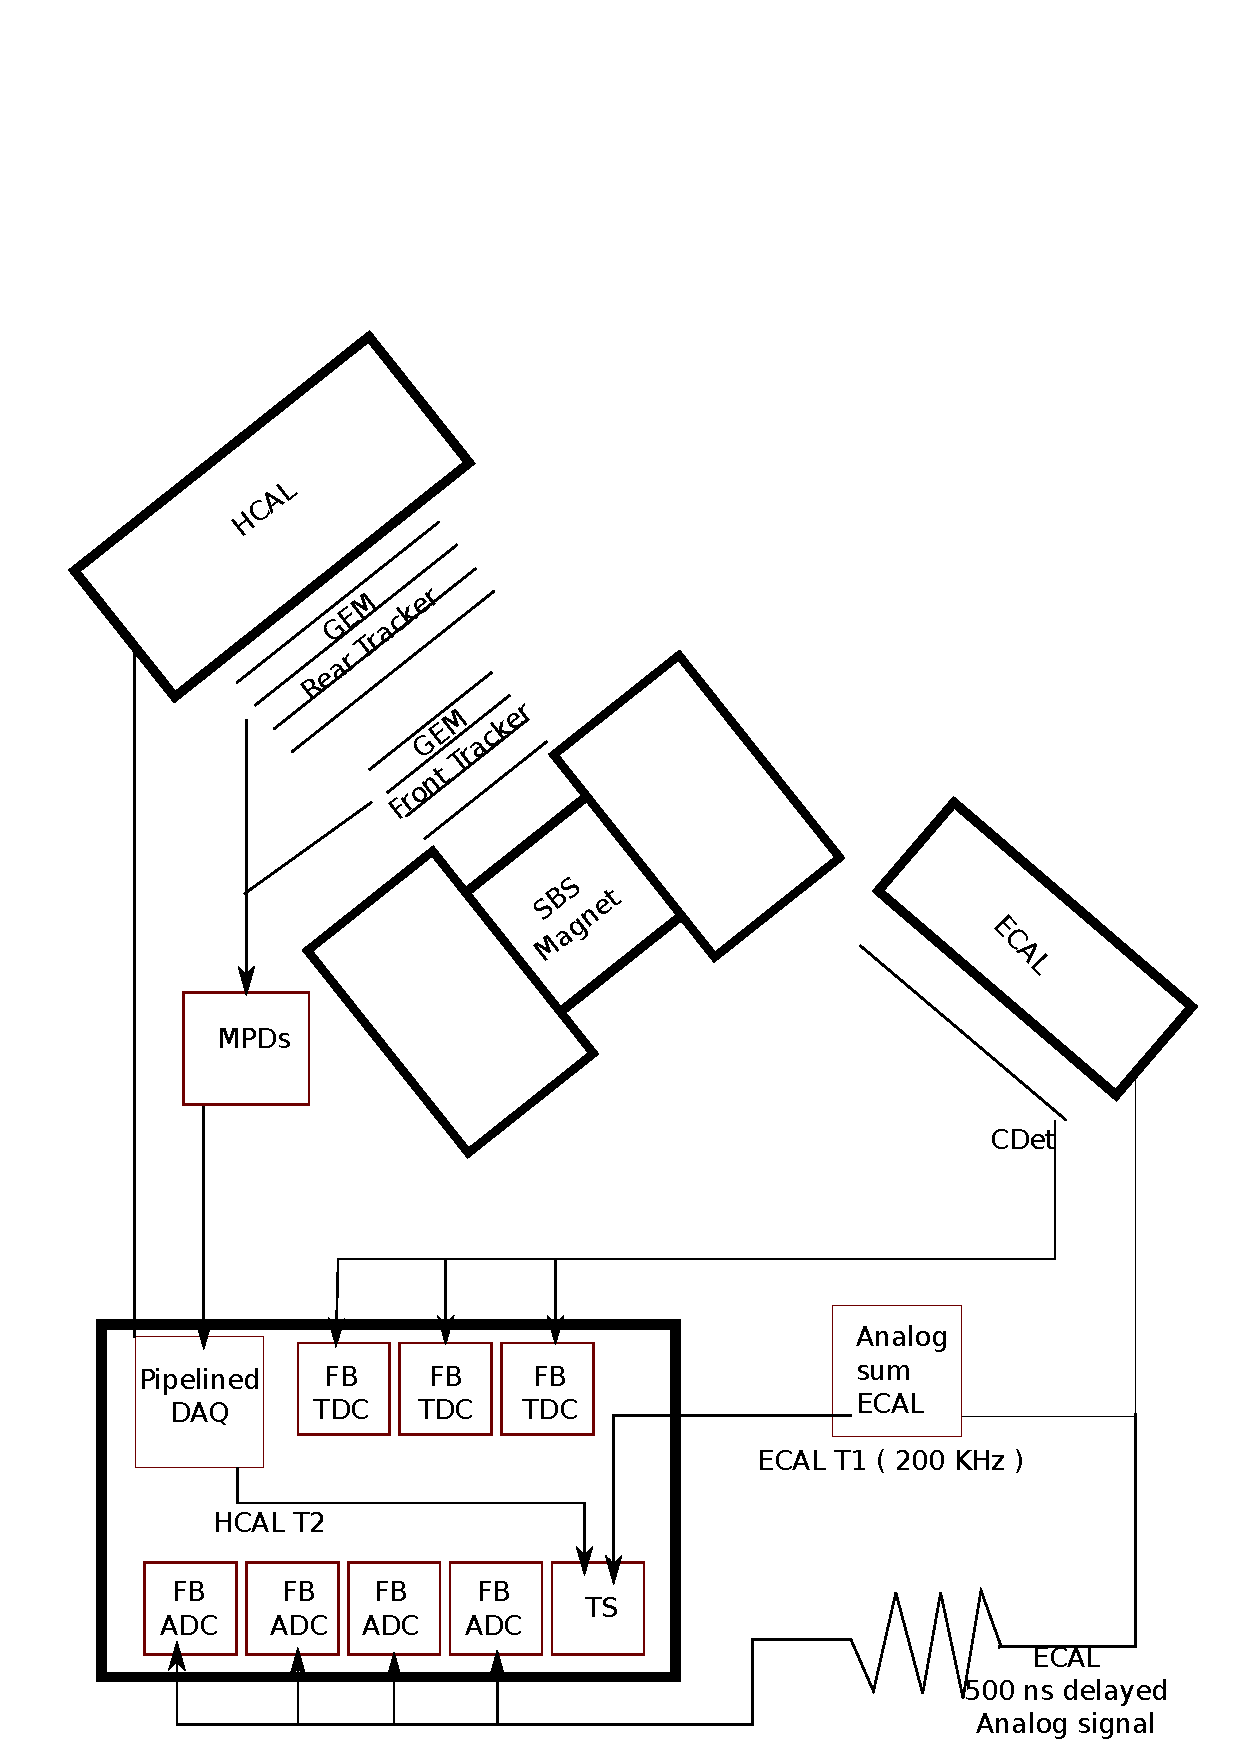
\includegraphics[scale=0.55]{figs/Gep5layout.pdf}\\
  \caption{GEp5 Layout}\label{fig:Gep5layout}

\end{figure}

\subsection {Expected data rates}
The expected trigger rate is 3 KHz. In order to be conservative the data rates will be evaluated for a 5 KHz rate.

\begin{table}
\begin{tabular}{|c|c|c|c|c|}
\hline
Detector & Channels & Modules & Event size (KB) & Data rate ( MB/s)\\
\hline
ECAL&1980&96&7.92&39.6\\
HCAL&288&18&11.52&57.6\\
CDET&2688&84&2.195&10.98\\
GEM FT&41472&24&25.05&127.18\\
GEM RT&61440&30&36.86&187.2\\
\hline
Total & & & & 422.6\\
\hline
\end{tabular}
\caption{Data rate for proton for factor experiments with only GEM pedestal suppression\label{GEpRateNoDeco}}
\end{table}

The GEM data is assumed with a 60\% occupancy of the detector right after common mode zero suppression. We assume that the deconvolution will reduce the data by a factor of 3 and that the geometrical correlation will reduce the GEM rate by at least another factor of 3. The actual data reduction factor will be evaluated using simulated data.
\begin{table}
\begin{tabular}{|c|c|c|c|c|}
\hline
Detector & Channels & Modules & Event size(KB) & Data rate ( MB/s)\\
\hline
ECAL&1980&96&7.92&39.6\\
HCAL&288&18&11.52&57.6\\
CDET&2688&84&2.195&10.98\\
GEM FT&41472&24&25.05&14.13\\
GEM RT&61440&30&36.86&20.8\\
\hline
Total & & & & 143.1\\
\hline
\end{tabular}
\caption{Data rate for proton for factor experiments with GEM deconvolution and geometrical matching\label{GEpRateDeco}}
\end{table}

The expected data rate of 143.1 MB/s is reasonable to record on tape. This rate assumed no zero suppression on ECAL and HCAL recording full waveform with 10 samples. Those can be set up to reduce further the data if needed.

\section{Neutron form factor overview}
\subsection {BigBite shower trigger}

\begin{figure}
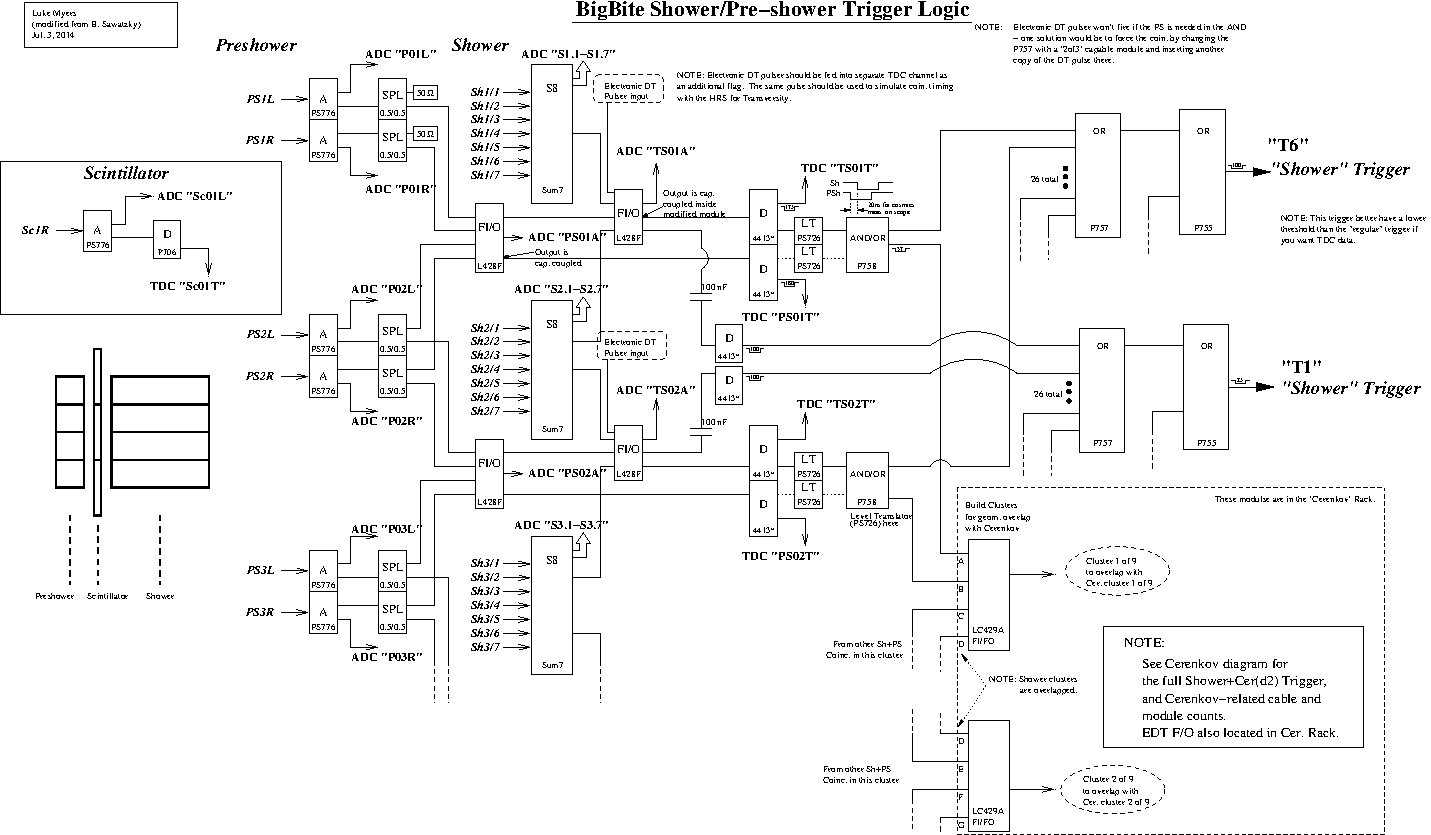
\includegraphics[scale=0.9,angle=270]{figs/Sh-PS_logic_v2A.pdf}\\
\caption {BigBite electron shower analog sum trigger \label{BBEtrig}}
\end{figure}

\label{sec:neutron-trig}
The GEn and GMn experiments will use the BigBite shower/preshower \ref{BBEtrig} as main trigger.
The shower calorimeter consist of an 7x27 array of  lead glass blocks. A preshower
 layer of 2x27 is placed in front of the shower. All shower rows are summed in sum of 7 modules, the each sum of seven is split and sent to a sum of four modules where it is added to another adjacent row in addition to the sum of the four preshower module in front of the two shower rows. The total sum of 2 rows of shower and 2 rows of preshower is discriminated and the shower trigger is formed when one of those sum is above threshold\ref{BBEtrig3D} .
It is expected to be less than 5 KHz so only one level of trigger is planned.
 If needed the coincidence could 
easily implemented as for GEp5.
\begin{figure}
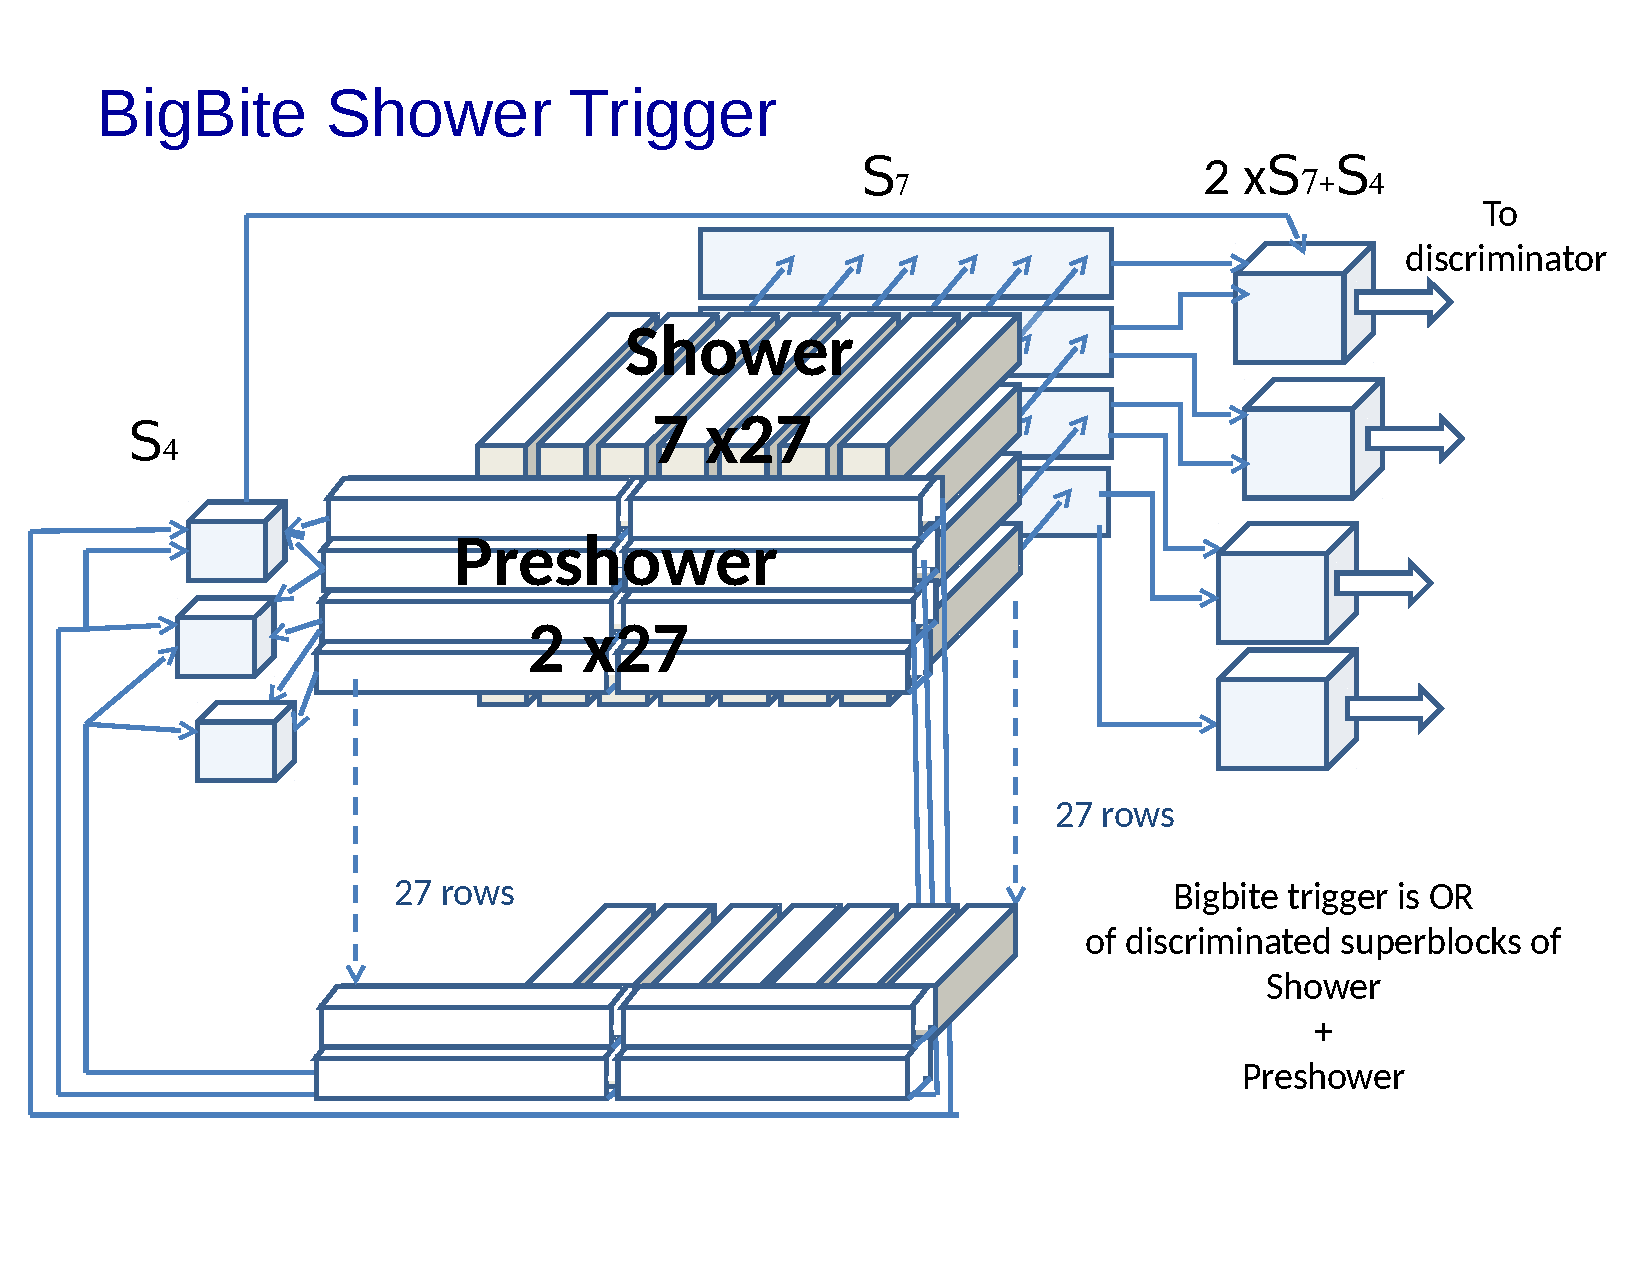
\includegraphics[scale=0.55]{figs/BBETrig3D.pdf}\\
\caption {Simplified BigBite electron shower analog sum trigger \label{BBEtrig3D}}
\end{figure}
The pipelined DAQ and GEM readout will be triggered by the L1 shower trigger directly.

\subsection {Overall setup}
A schematics of the DAQ system for the neutron form factors experiments can be found in Fig. \ref{fig:GENlayout}
and more details can be found the the GEn proposal \cite{GEnProp} and GMn proposal \cite{GMnProp}
\begin{figure}
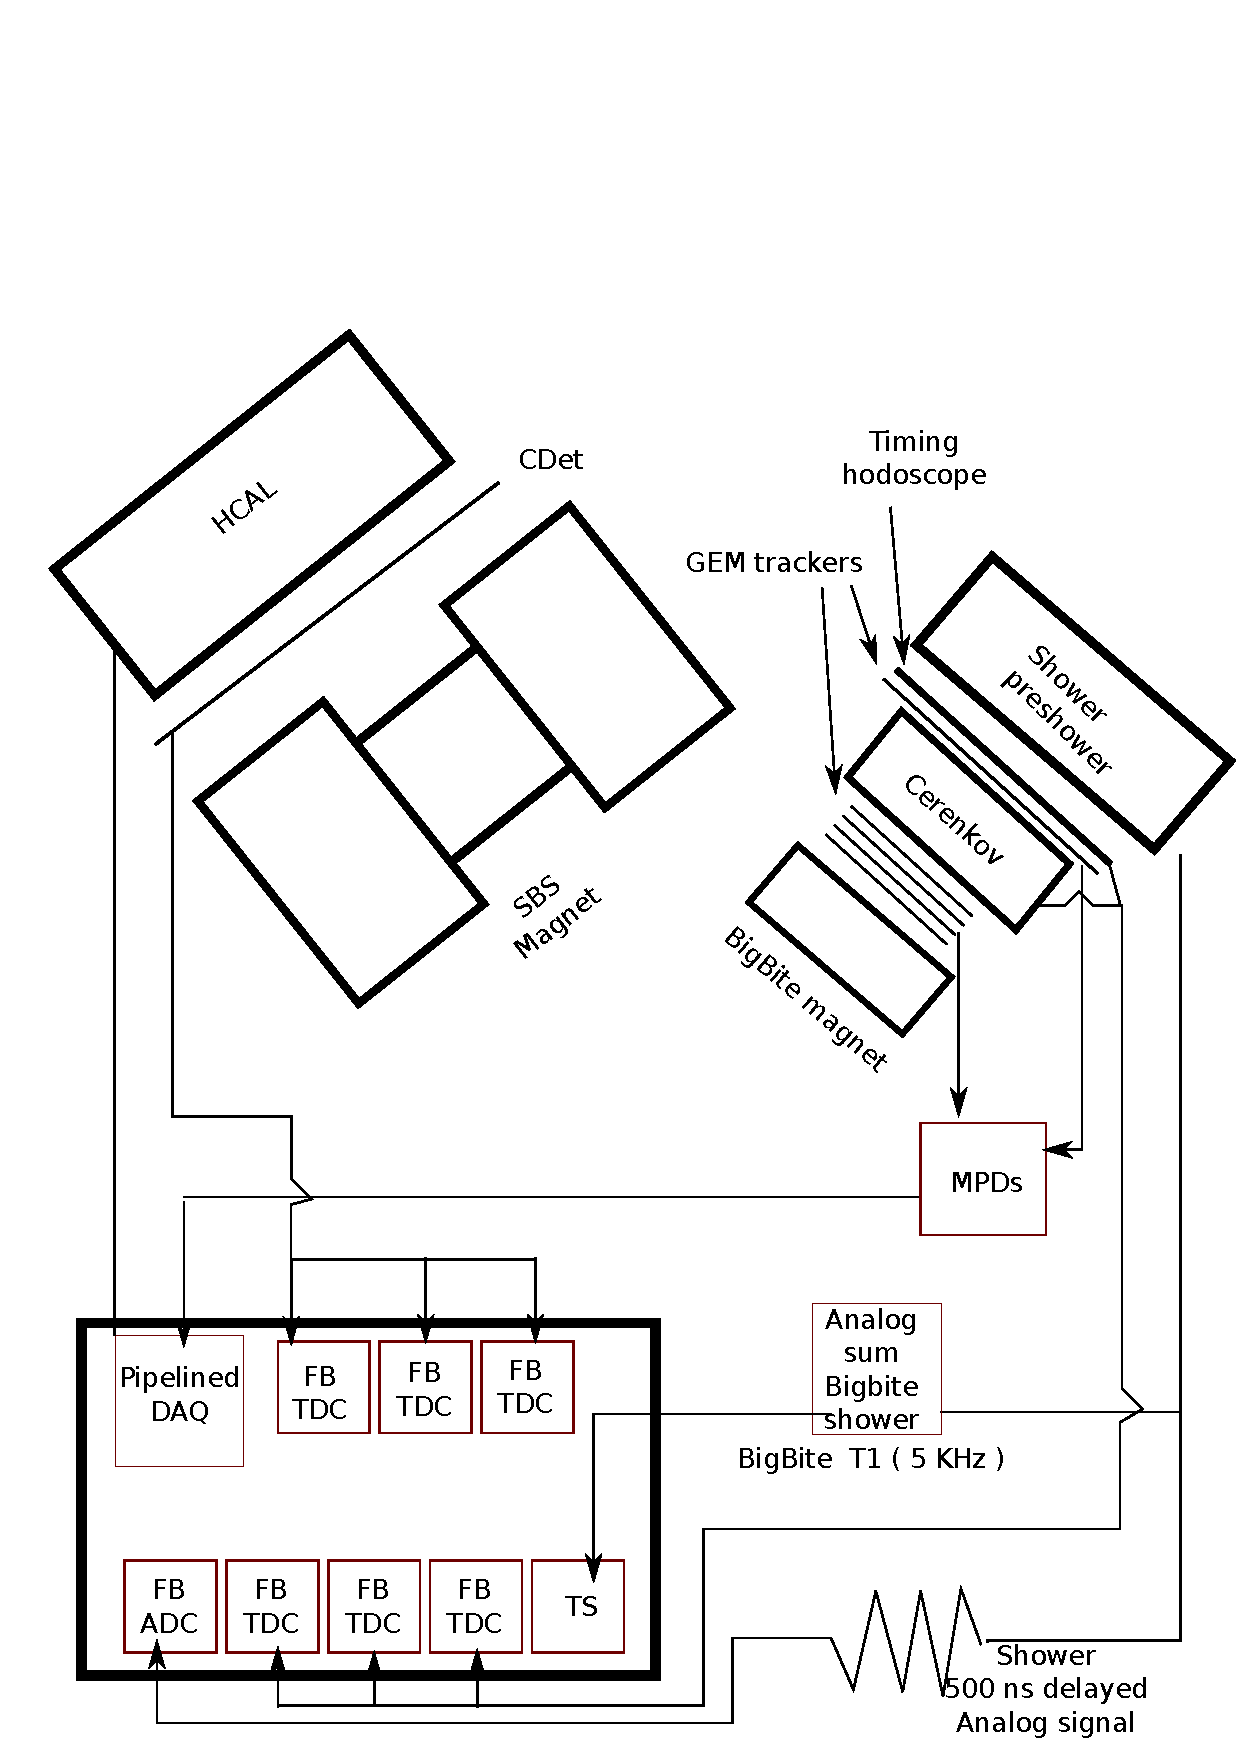
\includegraphics[scale=0.55]{figs/GeNlayout.pdf}\\
  \caption{GEn Layout}\label{fig:GENlayout}

\end{figure}
\subsection {Expected data rates}
\begin{table}
\begin{tabular}{|c|c|c|c|c|}
\hline
Detector & Channels & Modules & Event size (KB) & Data rate ( MB/s)\\
\hline
BB Shower&243&12&1.01&5.01\\
BB Cerenkov&510&18&0.42&2.08\\
BB Timing scint.&180&6&0.15&0.735\\
CDET&2688&84&2.195&10.98\\
HCAL&288&18&11.5&57.6\\
GEM FT&41472&24&25.05&127.18\\
GEM RT&6144&4&3.69&18.72\\
\hline
Total & & & & 222.3\\
\hline
\end{tabular}
\caption{Data rate for neutron for factor experiments without GEM deconvolution\label{GEnRateNoDeco}}
\end{table}
After deconvolution on the GEM data ( reduction by a factor of 3 )
\begin{table}
\begin{tabular}{|c|c|c|c|c|}
\hline
Detector & Channels & Modules & Event size (KB)  & Data rate ( MB/s)\\
\hline
BB Shower&243&12&1.01&5.01\\
BB Cerenkov&510&18&0.42&2.08\\
BB Timing scint.&180&6&0.15&0.735\\
CDET&2688&84&2.195&10.98\\
HCAL&288&18&11.5&57.6\\
GEM FT&41472&24&25.05&42.4\\
GEM RT&6144&4&3.69&6.24\\
\hline
Total & & & & 125.04\\
\hline
\end{tabular}
\caption{Data rate for neutron for factor experiments without GEM deconvolution\label{GEnRateDeco}}
\end{table}
We get similar data rates as for GEp5 dominated by the HCAL data which could be reduced by reading only time and amplitude instead of full waveform and implementing the pedestal suppression.
The GEM rate is low enough to have all the MPDs in one single VME64X crate.
Using the coincidence trigger could reduce further the data, we do not expect any issues as far as data rates are concerned for the neutron form factor experiments.

\section{Conclusion}
The DAQ acquistion for SuperBigBite is reusing older electronics to read out the ECAL, BigBite or the CDet.
In order to reach a design goal of 200 KHz of L1 with reasonable deadtime, a triple stand alone 
Fastbus DAQ will be used. Two GEM readout scheme were devised in addition to planning to implement
the deconvolution on the MPD readout itself, one through the standard VME64X bus with a maximum
transfer speed of about 100 MB/s which can be used when occupancy is low in the chamber.
The other one is a high speed transfer scheme where all the MPDs are readout in parallel using the optical link
and sent to a SSP module which can read up to 32 boards in parallel ( 32 GBit/s ) allowing an additionnal reduction of the data using geometrical constraints from other detectors.
Finally the pipeline electronics allows to easily make a clustering involving 4x4 blocks of the HCAL and will be used as L2 trigger for the GEp5 experiment.
Using the coincidence trigger, GEM deconvolution and geometrical matching we expect to have reasonable data rate for GEp5. The data rates are lower for the neutron form factor experiments thanks to a cleaner electron trigger coming from the BigBite spectrometer and are not an issue as well. 
The validation of the performance of the system will be done in 2015 with a small scale Fastbus/pipelined DAQ/ GEM readout setup.

\begin{thebibliography}{9}
\bibitem{GEpProp}E12-07-109: GEP/GMP   \url{http://hallaweb.jlab.org/collab/PAC/PAC34/PR-09-016-gen.pdf}
\bibitem{GEnProp}E12-09-016: GEN \url{ http://www.jlab.org/exp_prog/proposals/07/PR12-07-109.pdf}
\bibitem{GMnProp} E12-07-109: GEP/GMP \url{http://hallaweb.jlab.org/collab/PAC/PAC34/PR-09-019-gmn.pdf}
\bibitem{TIman} CODA TI board user manual\url{https://coda.jlab.org/wiki/Downloads/docs/manuals/VmeTIRManual.pdf}
\bibitem{TSman} CODA TS board user manual\url{ https://coda.jlab.org/wiki/Downloads/docs/manuals//ts_manual.pdf}
\bibitem{CODAman} CODA1.4 manual \url{https://coda.jlab.org/wiki/Downloads/docs/manuals//coda1.4.pdf}
%\cite{French:2001xb}
\bibitem{French:2001xb} 
  M.~J.~French, L.~L.~Jones, Q.~Morrissey, A.~Neviani, R.~Turchetta, J.~Fulcher, G.~Hall and E.~Noah {\it et al.},
  %``Design and results from the APV25, a deep sub-micron CMOS front-end chip for the CMS tracker,''
  Nucl.\ Instrum.\ Meth.\ A {\bf 466}, 359 (2001).
  %%CITATION = NUIMA,A466,359;%%
  %115 citations counted in INSPIRE as of 04 Nov 2014
\end{thebibliography}
\end{document}


\end{document}
